\chapter{Inverse ray mapping: numerical approach}
\label{chap:raymapping2}
In Chapter \ref{chap:raymapping1} we introduced an inverse method based on a ray mapping reconstruction in PS.
The goal was to calculate the intensity distribution at the target of optical systems. 
The idea was to construct a map from the target \point{T} to the source \point{S} using the PS of all the optical lines which are divided into several regions.  
The method developed in the previous chapter requires that the boundaries of the regions of every PS can be determined exactly. This is possible for systems formed by straight line segments.
The results found show that the procedure allows tracing the only rays located exactly on the boundaries of the regions with positive luminance. From these rays, \textit{exact} intensity was determined. \\ \indent
In this chapter we extend the method to systems formed by curved lines. In this case, the boundaries of the regions that form the PS cannot be determined exactly.
Because of this, we need to use a numerical procedure. In particular, we develop a method that employs only the PS of the target of the system. 
The boundaries are detected applying sequentially a bisection procedure in target PS and the inverse ray tracing.\\ \indent
In this chapter we test the method for two optical systems: the TIR-collimator and a parabolic reflector. The results are presented in Section \ref{sec:TIR} and \ref{sec:PR}, respectively.
\section{Explanation of the method}\label{sec:raymapping_explanation}
The purpose of this section is to present the generalized inverse ray mapping method valid for systems formed by curved lines. 
Given a partition $-1 = \variabile{p}^0<\variabile{p}^1<\cdots<\variabile{p}^{\nbin}$ of the interval $[-1,1]$ with $\nbin$ the number of rays in the partitioning, the intensity in target PS is given by Equation (\ref{eta2}) for every $\dir{}{}\in P$.
Therefore, the problem reduces to calculate the coordinates 
$\variabile{q}^{\textrm{\,min}}(\Pi, \variabile{p})$ and $\variabile{q}^{\textrm{\,max}}(\Pi, \variabile{p})$ of the rays on $\partial$\set{R}{}{}$(\Pi)$ for every path $\Pi$.\\ \indent 
We start from an intensity $I(p)=0$. Using the same idea of the inverse analytic ray mapping, for a given direction $\variabile{p}$, the procedure starts considering the end points $(\variabile{q}^{\,\textrm{a}}, \variabile{p})= (-\variabile{b}, \variabile{p})$ and $(\variabile{q}^{\,\textrm{b}}, \variabile{p}) = (\variabile{b}, \variabile{p})$ of \set{T}{}{} along direction $\variabile{p}$. We indicate with $\vect{r}_{\textrm{a}}$ and $\vect{r}_{\textrm{b}}$ the corresponding rays of these two points. Now, since the boundaries of the PS are unknown\footnote{More precisely, we know the boundaries of the region of the target PS but we cannot calculate exactly the boundaries of the other phase space.}, to understand from which line $\vect{r}_{\textrm{a}}$ and $\vect{r}_{\textrm{b}}$ are illuminated we apply the inverse ray tracing. We denote with $\nline$ the index of the target (line $\nline$) and with $\lineaj\in\{1,\cdots, \nline-1\}$ and $\lineak\in\{1,\cdots, \nline-1\}$ the lines from which $\vect{r}_{\textrm{a}}$ and $\vect{r}_{\textrm{b}}$ are emitted, respectively. $\Pi^\textrm{a} = (\lineaj, \nline)$ and $\Pi^\textrm{b} = (\lineak,\nline)$ are the paths followed by the two rays $\vect{r}_{\textrm{a}}$ and $\vect{r}_{\textrm{b}}$, respectively. In particular, $\vect{r}_{\textrm{a}}\in\partial$\set{R}{}{}$(\Pi^{\textrm{a}})$ and $\vect{r}_{\textrm{b}}\in\partial$\set{R}{}{}$(\Pi^{\textrm{b}})$ At this stage we know whether the two rays are emitted or not by the same line. \\ \indent 
If $\lineaj= \lineak$, then $\vect{r}_{\textrm{a}}$ and $\vect{r}_{\textrm{b}}$ hit the same line before reaching the target. 
In case $\lineaj = 1$ a possible path from the source to the target is found and the intensity is updated according to:
\begin{equation}
I(p) = I(p)+\variabile{q}^{\textrm{max}}(\Pi^\textrm{a}, \variabile{p})-\variabile{q}^{\textrm{min}}(\Pi^\textrm{a}, \variabile{p}),
\end{equation}
where $\variabile{q}^{\textrm{min}} = \min\{\variabile{q}^{\textrm{a}}, \variabile{q}^{\textrm{b}}\}$ and $\variabile{q}^{\textrm{max}} = \max\{\variabile{q}^{\textrm{a}}, \variabile{q}^{\textrm{b}}\}$. In case $\lineaj\neq1$ the two rays $\vect{r}_{\textrm{a}}$ and $\vect{r}_{\textrm{b}}$ are traced back again using the inverse ray tracing considering their corresponding coordinates on line $\lineaj$.
\\ \indent If $\lineaj\neq \lineak$ the rays $\vect{r}_\textrm{a}$ and $\vect{r}_\textrm{b}$ are emitted by two-different lines, hence $\Pi^{\textrm{a}}\neq \Pi^{\textrm{b}}$ and belong to different regions \set{R}{}{}$(\Pi^{\textrm{a}})$ and \set{R}{}{}$(\Pi^{\textrm{b}})$ in \set{T}{}{}. To determine the other rays on the boundary $\partial$\set{R}{}{}$(\Pi^{\textrm{a}})$, the bisection method is applied to the interval $[\variabile{q}^{\,\textrm{a}}(\Pi^{\textrm{a}}, \variabile{p}), \variabile{q}^{\,\textrm{b}}(\Pi^{\textrm{b}}, \variabile{p})]$ in target PS \set{T}{}{} along direction $\variabile{p}$. Thus, this interval is halves until the coordinates in target PS of the ray that follows the same path $\Pi^{\textrm{a}}$ of $\vect{r}_{\textrm{a}}$ are found. \\ \indent Bisection procedure continues until the length of the segment considered becomes smaller than a fixed tolerance. 
Giving as input the coordinates $\variabile{q}^{\,\textrm{a}}(\Pi^{\textrm{a}}, \variabile{p})$ and $\variabile{q}^{\,\textrm{b}}(\Pi^{\textrm{b}}, \variabile{p})$ of $\vect{r}_{\textrm{a}}$ and $\vect{r}_{\textrm{b}}$, the path $\Pi^\textrm{a}$ and the tolerance $\textrm{tol}= 10^{-12}$, the bisection method is implemented as in Algorithm \ref{alg:bisection}.
\begin{algorithm}
\caption{Bisection}\label{alg:bisection}
Initialize $\textrm{step} = 0$
\begin{algorithmic}[1]
\While {$|\variabile{q}^{\,\textrm{a}}-\variabile{q}^{\,\textrm{b}}|>\textrm{tol}$}
\State $\Pi^{\textrm{m}}\gets \nline,$
\State $\variabile{q}^{\,\textrm{m}}\gets \frac{\variabile{q}^{\,\textrm{a}}+\variabile{q}^{\,\textrm{b}}}{2},$ 
%\State $\variabile{p}^{\,\textrm{m}}\gets\variabile{p},$
\State $\vect{r}_{\textrm{m}}\gets \variabile{q}^{\,\textrm{m}}+s \variabile{p}$ with $s>0$ the arc-length,
\While {$\textrm{step}<\mbox{length}(\Pi^\textrm{a})-1$}
\State Trace back $\vect{r}_{\textrm{m}}$ considering its coordinates on line $\lineaj$,
\State Find the line $\lineak$ that the ray $\vect{r}_{\textrm{m}}$ hits.
\State $\Pi^{\textrm{m}}\gets (\lineak,\Pi^{\textrm{m}})$.
\If {$\lineak=1$ or $\lineak=\nline$}
\State $\textrm{step} = \mbox{length}(\Pi^\textrm{a})$ \Comment If the source or the target are reached \\  \Comment then exit from the while loop.
\Else \State $\textrm{step}\gets\textrm{step}+1$ 
\EndIf
\EndWhile
\If {$\Pi^\textrm{a} = \Pi^\textrm{m}$}
\State $(\variabile{q}^{\,\textrm{a}}, \variabile{p})\gets (\variabile{q}^{\,\textrm{m}}, \variabile{p})$
\State $\vect{r}_{\textrm{a}}\gets \vect{r}_{\textrm{m}}$
\Else 
\State $(\variabile{q}^{\,\textrm{b}}, \variabile{p})\gets (\variabile{q}^{\,\textrm{m}}, \variabile{p})$
\State $\vect{r}_{\textrm{b}}\gets \vect{r}_{\textrm{m}}$
\State $\Pi^\textrm{b}\gets \Pi^{\textrm{m}}$
\EndIf
\EndWhile
\State $(\variabile{q}^{\,\textrm{c}}, \variabile{p})\gets (\variabile{q}^{\,\textrm{a}}, \variabile{p}), \Pi^\textrm{c}\gets \Pi^{\textrm{a}}.$
\State $(\variabile{q}^{\,\textrm{d}}, \variabile{p})\gets (\variabile{q}^{\,\textrm{b}}, \variabile{p}), \Pi^\textrm{d}\gets \Pi^{\textrm{b}}.$
\State \Return $(\variabile{q}^{\,\textrm{c}}, \variabile{p})$, $(\variabile{q}^{\,\textrm{d}}, \variabile{p})$, $\Pi^{\textrm{c}}$ and $\Pi^{\textrm{d}}$.
\end{algorithmic}
\end{algorithm}
\\ \indent Once bisection stops, two points with coordinates $(\variabile{q}^{\,\textrm{c}}, \variabile{p})$ and $(\variabile{q}^{\,\textrm{d}}, \variabile{p})$ in \set{T}{}{} are found. The corresponding rays $\vect{r}_{\textrm{c}}$ and $\vect{r}_{\textrm{d}}$ follow path $\Pi^{\textrm{c}}=\Pi^{\textrm{a}}$ and $\Pi^{\textrm{d}}\neq\Pi^{\textrm{a}}$. 
All the rays with target coordinates $(\variabile{q}, \variabile{p})$ and $\variabile{q}^{\,\textrm{a}}\leq\variabile{q}\leq\variabile{q}^{\,\textrm{c}}$ follow path $\Pi = \Pi^{\textrm{a}}$, while the rays with target coordinates $(\variabile{q}, \variabile{p})$ with $\variabile{q}^{\,\textrm{d}}\leq\variabile{q}\leq\variabile{q}^{\,\textrm{b}}$ follow another path $\Pi \neq \Pi^{\textrm{a}}$ (see Figure \ref{fig:bisec}). 
%To clarify the procedure, in Figure \ref{fig:bisec} we show an example of target PS of an optical system where Algorithm \ref{alg:bisection} is run for the interval $[\variabile{q}^{\textrm{a}}, \variabile{q}^{\textrm{b}}]$ along direction $\variabile{p}=0$. Applying bisection the coordinates $(\variabile{q}^{\textrm{c}}(\variabile{p}), \variabile{p})$ and $(\variabile{q}^{\textrm{d}}(\variabile{p}), \variabile{p})$ of two points are found. The corresponding rays follow the paths $\Pi^{\textrm{c}}$ and $\Pi^{\textrm{d}}$, where $\Pi^{\textrm{c}}= \Pi^{\textrm{a}}\neq\Pi^{\textrm{d}}$. If $\Pi^{\textrm{c}}$ is a path from the source to the target, Algorithm \ref{alg:bisection} is applied to the sub-interval 
%$[\variabile{q}^{\textrm{a}}(\variabile{p}), \variabile{q}^{\textrm{c}}(\variabile{p})]$, otherwise the it is applied again to the sub-interval $[\variabile{q}^{\textrm{d}}(\variabile{p}), \variabile{q}^{\textrm{b}}(\variabile{p})]$. The bisection procedure is repeated for all the sub-intervals found along direction $\variabile{p}$, until the entire interval $[\variabile{q}^{\textrm{a}}(\variabile{p}), \variabile{q}^{\textrm{c}}(\variabile{p})]$ is investigated.
\begin{figure}[h]
  \begin{center}
  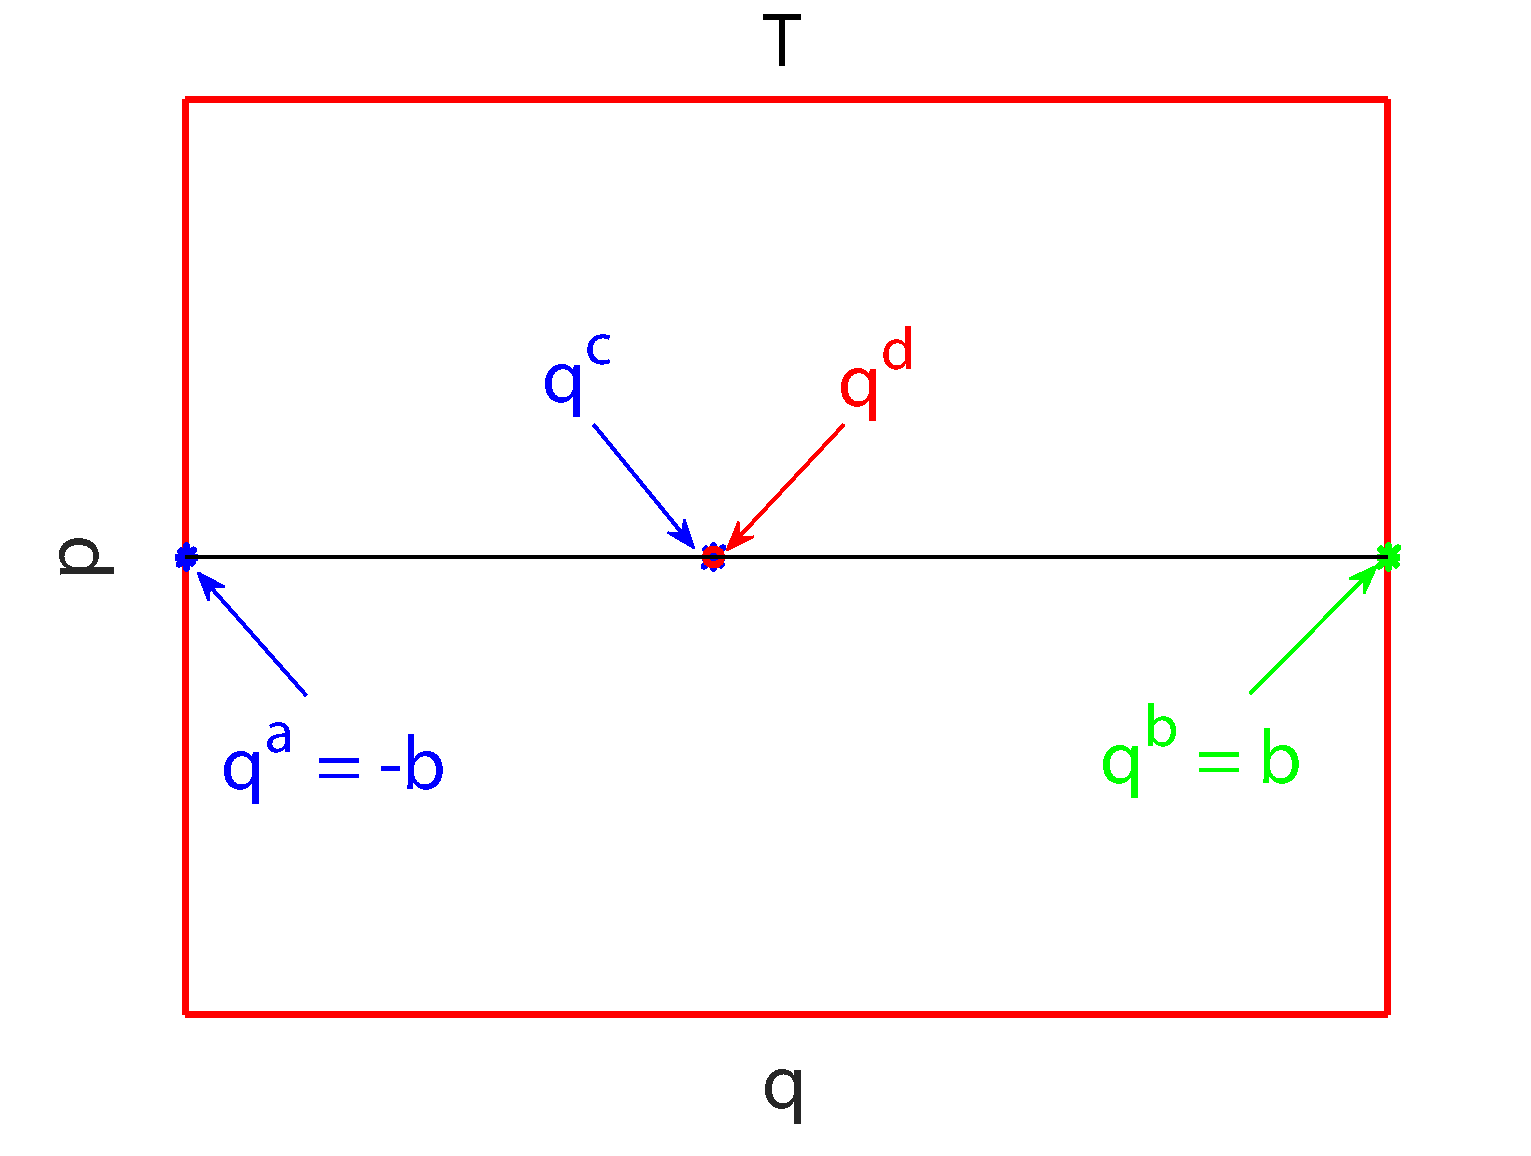
\includegraphics[width=0.7\textwidth]{T4_1_example}
  \end{center}
  \caption{\textbf{Bisection in target PS \set{T}{}{}.} Algorithm \ref{alg:bisection} is run for the interval $[\variabile{q}^{\textrm{a}}, \variabile{q}^{\textrm{b}}]$ along direction $\variabile{p}=0$. The coordinates $\variabile{q}^{\textrm{c}}$ and $\variabile{q}^{\textrm{d}}$ are found such that 
$|\variabile{q}^{\textrm{c}}-\variabile{q}^{\textrm{d}}|<\textrm{tol}$. $\Pi^{\textrm{c}}= \Pi^{\textrm{a}}$ and $\Pi^{\textrm{d}}\neq \Pi^{\textrm{a}}$.}
\label{fig:bisec}
 \end{figure}
\\ \indent Now, if $\lineaj\neq1$ the procedure applied to the interval 
$[\variabile{q}^{\textrm{a}}(\variabile{p}), \variabile{q}^{\textrm{b}}(\variabile{p})]$ needs to be applied to $[\variabile{q}^{\textrm{a}}(\variabile{p}),\variabile{q}^{\textrm{c}}(\variabile{p})]$ until the source is reached, i.e. until $\lineaj=1$. If $\lineaj=1$, the source is reached by the rays traced back from the target. This means that a possible path $\Pi$ from \point{S} to \point{T} is found and the position coordinates $\variabile{q}^{\textrm{\,min}}(\Pi, \variabile{p})$ and $\variabile{q}^{\textrm{\,max}}(\Pi, \variabile{p})$ on \set{T}{}{} of the rays located at the boundaries $\partial$\set{R}{}{}$(\Pi)$ of the rays that follow that path are determined. \\ \indent 
Finally, to detect all the possible paths that can occur along direction $\variabile{p}$ the procedure explained above is applied also to the interval $[\variabile{q}^{\textrm{d}}(\variabile{p}), \variabile{q}^{\textrm{b}}(\variabile{p})]$ along direction $\variabile{p}$. 
The main steps of the method are outlined in the following.
\begin{enumerate}
\item Given a direction \variabile{p}, consider the end points $(\variabile{q}^{\,\textrm{a}}, \variabile{p}^{\,\textrm{a}})$ and $(\variabile{q}^{\,\textrm{b}}, \variabile{p}^{\,\textrm{a}})$ of the target PS \set{T}{}{}, where $\variabile{q}^{\,\textrm{a}} = -\variabile{b}$, $\variabile{q}^{\,\textrm{b}} = \variabile{b}$ and $\variabile{p}^{\,\textrm{a}} = \variabile{p}^{\,\textrm{b}} = \variabile{p}$. Star from $\lineai=\nline$
\item \label{ray trace} Trace back the rays $\vect{r}_{\textrm{a}}$ and $\vect{r}_\textrm{b}$ corresponding to the coordinates  $(\variabile{q}_{\lineai}^{\,\textrm{a}}, \variabile{p}_{\lineai}^{\,\textrm{a}})$ and $ (\variabile{q}_{\lineai}^{\,\textrm{b}}, \variabile{p}_{\lineai}^{\,\textrm{b}})$ using the inverse ray tracing procedure
\footnote{If $\lineai=\nline $ then $\variabile{p}_{\lineai}^{\,\textrm{a}}=\variabile{p}_{\lineai}^{\,\textrm{b}}=\variabile{p}$, otherwise $\variabile{p}_{\lineai}^{\,\textrm{a}}\neq\variabile{p}_{\lineai}^{\,\textrm{b}}$},
\item Determine indices $\lineaj\neq\lineai$ and $\lineak\neq\lineai$ of the lines that  $\vect{r}_{\textrm{a}}$ and $\vect{r}_{\textrm{b}}$  hit.\\
\item Update the paths $\Pi^\textrm{a}$ and $\Pi^\textrm{b}$ of rays $\vect{r}_\textrm{a}$ and $\vect{r}_\textrm{b}$.  $\Pi^\textrm{a} = (\lineaj, \Pi^{\textrm{a}})$ and $\Pi^\textrm{b} = (\lineak, \Pi^\textrm{b}),$
\item If $\lineaj=\lineak \neq 1$ \& $\lineaj=\lineak \neq \nline$
\begin{itemize}
\item $\lineai=\lineaj$,
%\item Consider the coordinates of rays $\vect{r}_{\textrm{a}}$ and $\vect{r}_{\textrm{b}}$ on line $\lineaj$ 
\item Restart the procedure from point $\ref{ray trace}$, 
\end{itemize}
\item If $\lineaj=\lineak= 1$ 
\begin{itemize}
\item A relevant path $\Pi^{\textrm{a}} = \Pi^{\textrm{b}}$ is found. 
\item Determine 
\begin{equation*}
\begin{aligned}
\variabile{q}^{\textrm{min}}(\Pi^{\textrm{a}}, \variabile{p})&=\min\{\variabile{q}^{\textrm{a}}(\Pi^{\textrm{a}}, \variabile{p}), \variabile{q}^{\textrm{b}}(\Pi^{\textrm{b}}, \variabile{p})\}\\ 
\variabile{q}^{\textrm{max}}(\Pi^{\textrm{a}}, \variabile{p})&=\max\{\variabile{q}^{\textrm{a}}(\Pi^{\textrm{a}}, \variabile{p}), \variabile{q}^{\textrm{b}}(\Pi^{\textrm{b}}, \variabile{p})\},
\end{aligned}
\end{equation*}
\item Update the intensity $$I(\variabile{p}) = I(p)+\variabile{q}^{\textrm{max}}(\Pi^{\textrm{a}}, \variabile{p})-\variabile{q}^{\textrm{min}}(\Pi^{\textrm{a}}, \variabile{p})$$
\end{itemize}
%\item If $\lineaj=\lineak= \nline$ stop the procedure (the rays reach the target again).
\item If $\lineaj\neq\lineak$ 
\begin{itemize}
\item Apply the bisection method to the interval $[\variabile{q}^{\textrm{a}}, \variabile{q}^{\textrm{b}}]$ along direction $\variabile{p}$.
\item Find the points with coordinates $(\variabile{q}^{\,\textrm{c}}, \variabile{p})$ and $(\variabile{q}^{\,\textrm{d}}, \variabile{p})$ in target PS \set{T}{}{} where $|\variabile{q}^{\,\textrm{c}}-\variabile{q}^{\,\textrm{d}}|<\textrm{tol}$ and $\textrm{tol}=10^{-12}$ is the tolerance in the bisection procedure. 
\item If $\lineaj\neq\nline$
\begin{itemize}
\item Update $(\variabile{q}^{\textrm{b}}, \variabile{p}) = (\variabile{q}^{\textrm{c}}, \variabile{p})$,
\item Update $(\variabile{q}_{\lineaj}^{\textrm{b}}, \variabile{p}_{\lineaj}^{\textrm{b}}) = (\variabile{q}_{\lineaj}^{\textrm{c}}, \variabile{p}_{\lineaj}^{\textrm{b}})$,

\item $\lineai = \lineaj$

\item Restart from $\ref{ray trace}$ with the updated coordinates,
\end{itemize}
\item Update $(\variabile{q}^{\textrm{a}}, \variabile{p} )= (\variabile{q}^{\textrm{d}}, , \variabile{p})$,
\item $\Pi^{\textrm{a}} = \Pi^{\textrm{c}}$
\item Update $(\variabile{q}_{\lineaj}^{\textrm{a}}, \variabile{p}_{\lineaj}^{\textrm{a}}) = (\variabile{q}_{\lineaj}^{\textrm{d}}, \variabile{p}_{\lineaj}^{\textrm{d}})$,
\item Restart from $\ref{ray trace}$, 

\end{itemize}

\end{enumerate}
Giving as input $I(\variabile{p})=0$ for every direction $\variabile{p}$ and the tolerance $\textrm{tol}=10^{-12}$,
the method is developed using the recursive Algorithm \ref{alg:recursiveraymapping}.
% Insert algorithm
\begin{algorithm}
\caption{Recursive function for the extended ray mapping}\label{alg:recursiveraymapping}
Initialize $\lineai = \nline$, $\variabile{q}^{\,\textrm{a}}= \variabile{q}^{\,\textrm{a}}_{\lineai}=-\variabile{b}$, $\variabile{q}^{\,\textrm{b}}= \variabile{q}^{\,\textrm{b}}_{\lineai}=\variabile{b}$, $\dir{}{}=\variabile{p}^{\textrm{a}}_\lineai=\variabile{p}^{\textrm{b}}_\lineai=\textrm{const}$, $\Pi^{\textrm{a}}=({\nline})$.
\begin{algorithmic}[1]
\Procedure {Intensity computation}{$\variabile{q}^{\,\textrm{a}}$,  $\variabile{q}^{\,\textrm{b}}$, $\variabile{q}^{\,\textrm{a}}_{\lineai},$  $\variabile{q}^{\,\textrm{b}}_{\lineai},$ $\dir{}{}$, $\variabile{p}^{\textrm{a}}_{\lineai}$, $\variabile{p}^{\textrm{b}}_{\lineai}$, $\Pi^{\textrm{a}}$, $\lineai$}
\State Apply the inverse ray tracing to the coordinates $(\variabile{q}^{\,\textrm{a}}_{\lineai},\variabile{p}^{\textrm{a}}_{\lineai})$ and $(\variabile{q}^{\,\textrm{b}}_{\lineai},\variabile{p}^{\textrm{b}}_{\lineai})$ on $\lineai$ of $\vect{r}_{\textrm{a}}$ and $\vect{r}_{\textrm{b}}$.
\State Find the lines $\lineaj\neq\lineai$ and $\lineak\neq\lineai$ from which $\vect{r}_{\textrm{a}}$ and $\vect{r}_{\textrm{b}}$ are emitted, respectively.
\State Update path $\Pi^{\textrm{a}}\gets(\lineaj, \Pi^{\textrm{a}})$
\State Calculate the coordinates $(\variabile{q}^{\,\textrm{a}}_{\lineaj},\variabile{p}^{\textrm{a}}_{\lineaj})$ and $(\variabile{q}^{\,\textrm{b}}_{\lineaj}, \variabile{p}^{\textrm{b}}_{\lineaj})$ on line $\lineaj$
\If {$\lineaj = \lineak$}
\If{$\lineaj\neq1$}
\State\Return{\Call{Intensity computation}{$\variabile{q}^{\,\textrm{a}},$  $\variabile{q}^{\,\textrm{b}},$ $\variabile{q}^{\,\textrm{a}}_{\lineaj},$ $\variabile{q}^{\,\textrm{b}}_{\lineaj},$ $\dir{}{}$, $\variabile{p}^{\textrm{a}}_{\lineaj}$, $\variabile{p}^{\textrm{b}}_{\lineaj}$, $\Pi^{\textrm{a}}$, $\lineaj$}}
\Else { \State Calculate
$\variabile{q}^{\textrm{min}} = \min\{\variabile{q}^{\textrm{a}}, \variabile{q}^{\textrm{b}}\}$ and $\variabile{q}^{\textrm{max}} = \max\{\variabile{q}^{\textrm{a}}, \variabile{q}^{\textrm{b}}\}$
\State $I(\dir{}{}) = I(\dir{}{})+\variabile{q}^{\textrm{max}}(\Pi^{\textrm{a}}, \dir{}{})
-\variabile{q}^{\textrm{min}}(\Pi^{\textrm{a}}, \dir{}{}),$}
\EndIf
\Else 
\State Apply bisection to the segment $[\variabile{q}^{\,\textrm{a}}(\Pi^\textrm{a}, \dir{}{}), \variabile{q}^{\,\textrm{b}}(\Pi^\textrm{b}, \dir{}{})]$
\State Find the target coordinates $(\variabile{q}^{\,\textrm{c}},\variabile{p})$ and $(\variabile{q}^{\,\textrm{d}},\variabile{p})$ of the rays $\vect{r}_{\textrm{c}}$ and $\vect{r}_{\textrm{d}}$, where $|\variabile{q}^{\,\textrm{c}}-\variabile{q}^{\,\textrm{d}}|<\textrm{tol}$
\If {$\lineaj\neq \nline$}
\State\Return{\Call{Intensity computation}{$\variabile{q}^{\,\textrm{a}},$  $\variabile{q}^{\,\textrm{c}},$ $\variabile{q}^{\,\textrm{a}}_{\lineaj},$ $\variabile{q}^{\,\textrm{c}}_{\lineaj},$ $\dir{}{}$, $\variabile{p}^{\textrm{a}}_{\lineaj}$, $\variabile{p}^{\textrm{c}}_{\lineaj}$, $\Pi^{\textrm{a}}$, $\lineaj$}}
\EndIf 
\State\Return{\Call{Intensity computation}{$\variabile{q}^{\,\textrm{d}},$  $\variabile{q}^{\,\textrm{b}},$ $\variabile{q}^{\,\textrm{d}}_{\lineaj},$ $\variabile{q}^{\,\textrm{b}}_{\lineaj},$ $\dir{}{}$, $\variabile{p}^{\textrm{d}}_{\lineaj}$, $\variabile{p}^{\textrm{b}}_{\lineaj}$, $\Pi^{\textrm{d}}$, $\lineaj$}}
\EndIf
\State \EndProcedure
\end{algorithmic}
\end{algorithm}
\\ \indent The explained procedure is able to determine all the possible paths that the rays can follow during their propagation from \set{S}{}{} to \set{T}{}{}. Also, the rays located on the boundaries of the regions with positive luminance on target PS \set{T}{}{} are found.\\ \indent
Next, the method is applied to two optical systems formed by curved lines. In the next section we show the results for the TIR-collimator.
\section{Results for the TIR-collimator}\label{sec:TIR}
% Introduction 
In this section we apply the extended inverse ray mapping to the TIR-collimator presented in Chapter \ref{chap:boundaries_alpha} and depicted in Figure \ref{fig:analyticlens}. The target PS of this system is the rectangular \set{T}{}{}$= [-\variabile{b}, \variabile{b}]\times[-1,1]$ with $\variabile{b}=9.7$. The aim is to detect all the possible path $\Pi$ and the rays located on the boundaries $\partial$\set{R}{}{}$(\Pi)$ of the corresponding regions in target PS. 
\\ \indent In Chapter \ref{chap:boundaries_alpha}, we found five different paths for the the TIR-collimator. The boundaries of the corresponding regions in target PS \set{T}{}{} are in general difficult to approximate. Furthermore, along the same direction $\dir{}{}$ more than two points can be located on the boundary $\partial$\set{R}{}{}$(\Pi)$ of the region \set{R}{}{}$(\Pi)$ corresponding to a certain path $\Pi$. To determine properly all the boundaries 
$\partial$\set{R}{}{}$(\Pi)$, we need to divide the interval $[-\variabile{b}, \variabile{b}]$ in 
\set{T}{}{} into intervals of the same length (bins). Hence, we consider a partitioning 
$Q = -\variabile{b}=\variabile{q}^{0}<\variabile{q}^{1}<\cdots<\variabile{q}^{\textrm{Ni}}=\variabile{b}$ of $[-\variabile{b}, \variabile{b}]$ where $\textrm{Ni}$ is the total number of bins along the $\variabile{q}$-axis.
For each direction $\dir{}{}\in [-1,1]$ the procedure explained in Section \ref{chap:raymapping2} is repeated for every sub-interval $[\variabile{q}^{\textrm{k}}(\dir{}{}), \variabile{q}^{\textrm{k}+1}(\dir{}{})]\subset [\variabile{q}^{\textrm{a}}(\dir{}{}), \variabile{q}^{\textrm{b}}(\dir{}{})]$ with $\textrm{k}=0, \cdots, \textrm{Ni}-1$ and $\variabile{q}^{\textrm{a}}(\dir{}{}) = -\variabile{b}$ and $\variabile{q}^{\textrm{b}}(\dir{}{}) = \variabile{b}$.\\ \indent
To establish in how many bins \textrm{Ni} we need to divide the target, we exploit \'{e}tendue conservation. We use the same idea applied to determine the value of $\alpha$ for $\alpha$-shapes methods and to provide a stopping criterion for the triangulation refinement (see Chapters \ref{chap:boundaries_alpha} and \ref{chap:triangulation}). 
The source \'{e}tendue $U_1$ is calculated from Equation (\ref{eq:Usource}) obtaining, for the TIR-collimator, $U_1 \approx 7.7$. The target \'{e}tendue $U_\textrm{t}$ is given by Equation (\ref{eq:etenduetarg1}). $U_\textrm{t}$ is calculated several times considering every time a different partitioning $Q$ for the $\variabile{q}$-axis of the target PS. Next, the absolute value of the difference between the source and target \'{e}tendue is obtained from
\begin{equation}\label{eq:delta_raymapping}
\Delta U =  \big|U_1-U_{\textrm{t}}\big|.
\end{equation}
If a small value of $\Delta U$ is obtained, then a good approximation of $U_{\textrm{t}}$ is found and therefore, the partition $Q$ used for the computation of $U_{\textrm{t}}$ is suitable for detecting correctly the boundaries $\partial$\set{R}{}{}$(\Pi)$. In Figure \ref{fig:etendue_raymapping_tir} we show how $\Delta U$ decreases by increasing the number of bins $\textrm{Ni}$ in the partitioning $Q$.  
\begin{figure}[h]
  \begin{center}
  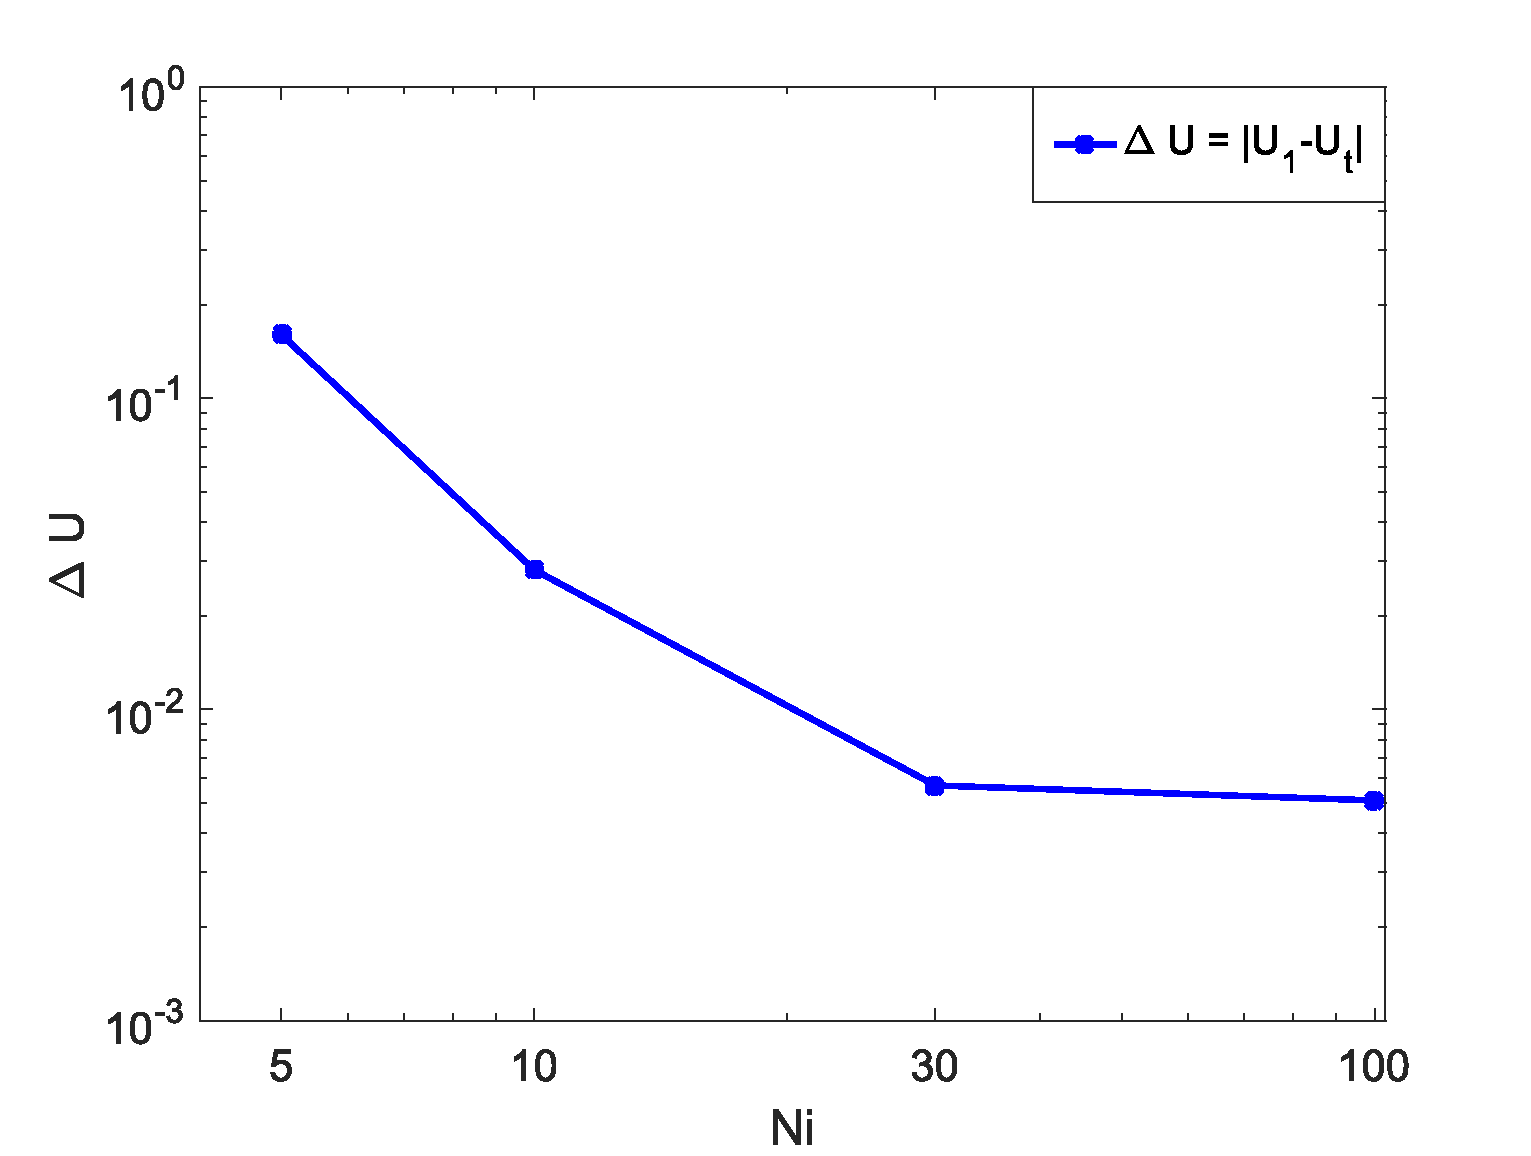
\includegraphics[width=0.7\textwidth]{etendue_raymapping_tir}
  \end{center}
  \caption{\textbf{Difference between the source and the target \'{e}tendue for the TIR-collimator.}
 $U_1$ is calculated from Equation (\ref{eq:Usource}). $U_{\textrm{t}}$ is computed four times increasing every time the number of bins $\textrm{Ni}$ where $\textrm{Ni}=\{5,10,30,100\}$. }
\label{fig:etendue_raymapping_tir}
 \end{figure}
In Figure \ref{fig:boundaries_TIR_ray_mapping} we show the distribution of the rays traced using the inverse ray mapping method with $\textrm{Ni}=30$ and $\nbin = 100.$ 
\begin{figure}[h]
  \begin{center}
  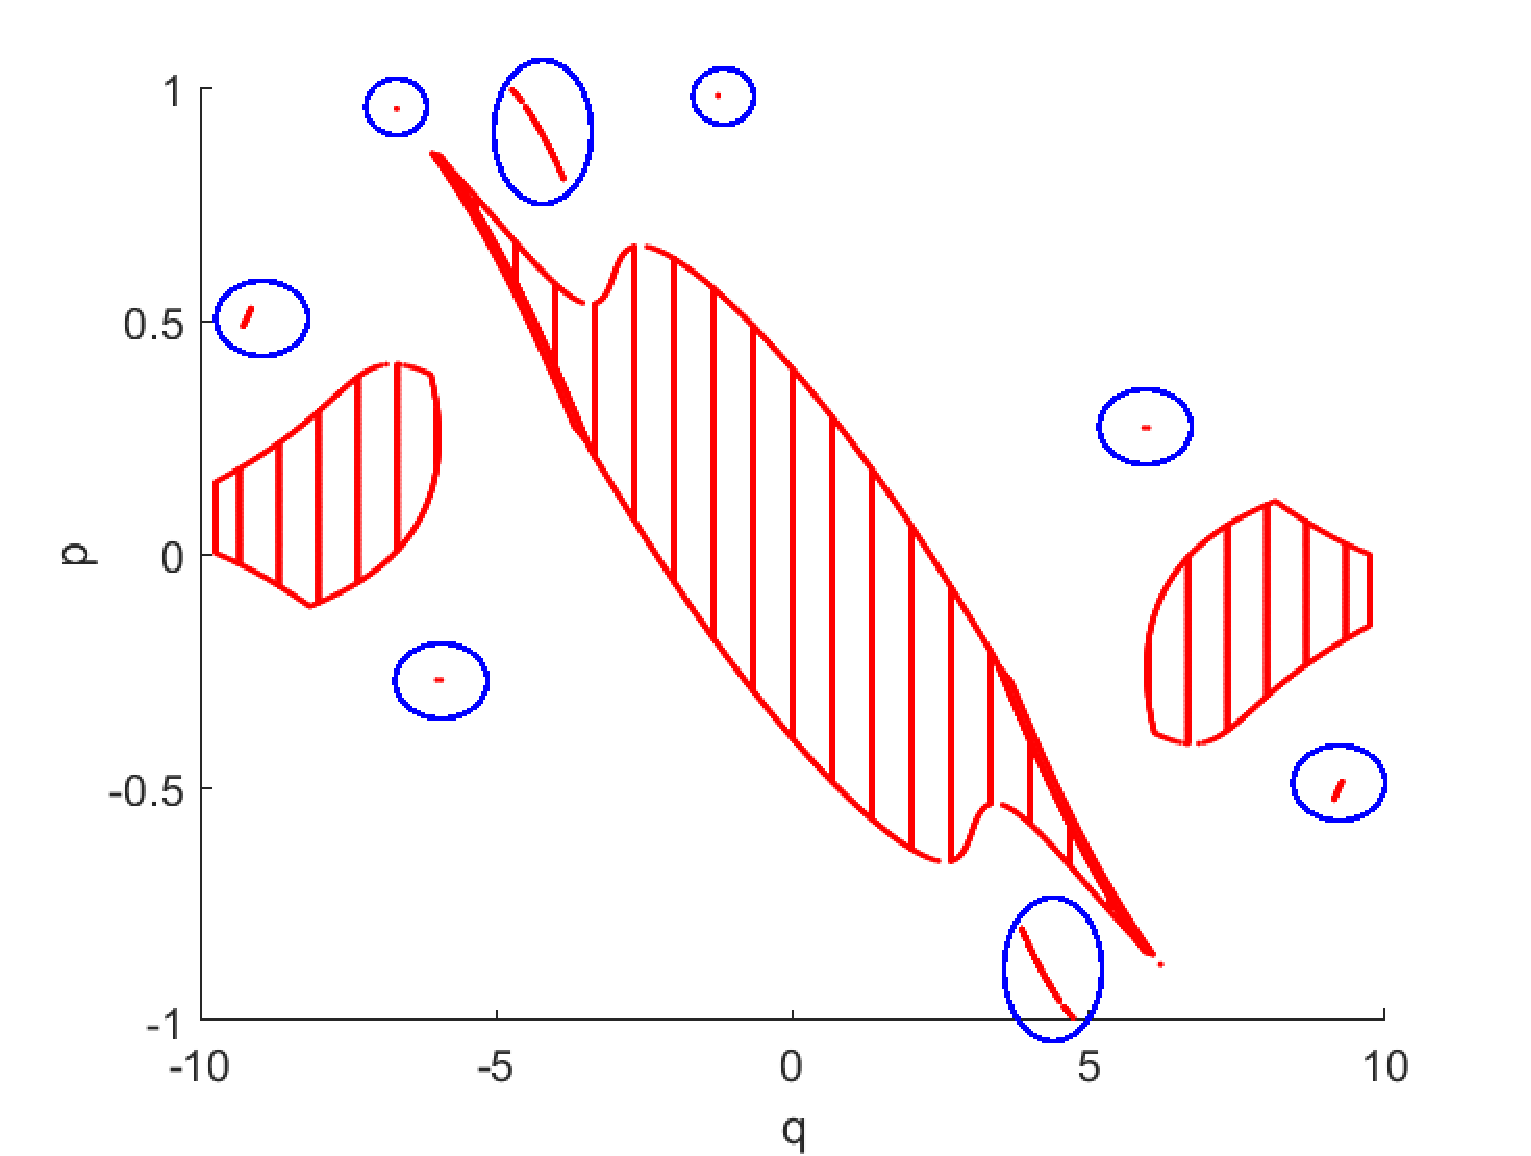
\includegraphics[width=0.7\textwidth]{boundaries_ray_mapping_tir}
  \end{center}
  \caption{\textbf{Rays distribution at target PS of the TIR-collimator.}
 The $\variabile{q}$-axis is divided into $\textrm{Ni}=30$ bins, the $\variabile{p}$-axis is divided into $\nbin = 100$ bins. Using the ray mapping method only few rays are traced from the target to the source (red dots). Because of numerical error, few rays outside the region with positive luminance are found (Rays rimmed in red).}
\label{fig:boundaries_TIR_ray_mapping}
 \end{figure}
In this case, the inverse ray mapping detects $11$ different paths from the source to the target. 
We observe that only $5$ of them are the paths that we expected from PS ray tracing (see Chapter \ref{chap:boundaries_alpha}). 
The inverse ray mapping also detect the following paths:
\begin{equation}\label{eq:paths_tir}
\begin{array}{llll}
\Pi_6&=(1,2,9,8,7,12), & \Pi_7&=(1,2,5,6,7,12), \\
\Pi_8&=(1,2,2,7,12),& \Pi_9&=(1,7,12),\\
\Pi_{10}&=(1,2,4,6,7,12),& \Pi_{11}&=(1,2,10,8,7,12).
\end{array}\end{equation}
Those paths are due to numerical error, the rays that follow this path are rimmed in blue in Figure \ref{fig:boundaries_TIR_ray_mapping}. The numerical error can be related to the precision of the bisection method and the inverse ray tracing. We remark that in the inverse ray tracing, the intersection between the ray and the lens (line $2$) is computed using the Newton-Raphson procedure.
To detect only the boundaries of the regions formed by the rays that follow the \textit{physical} $\Pi_{\variabile{j}}$, with $\variabile{j}\in\{1, \cdots, 5\}$, we check the index of refraction that every ray has once it arrives at the source.
If this is equal to the same index of \point{S} ($\n=1$ for the TIR-collimator), then the ray follows a physical path, otherwise it follows one of the paths in (\ref{eq:paths_tir}) and, therefore, it is not considered for the intensity calculation. This gives the rays distribution at the target PS shown in Figure \ref{fig:boundaries_TIR_ray_mapping1} where $\textrm{Ni}=30$. We observe that, discarding those rays, $5$ different paths are found. These are the same paths we obtained using PS ray tracing.
\begin{figure}[h]
  \begin{center}
  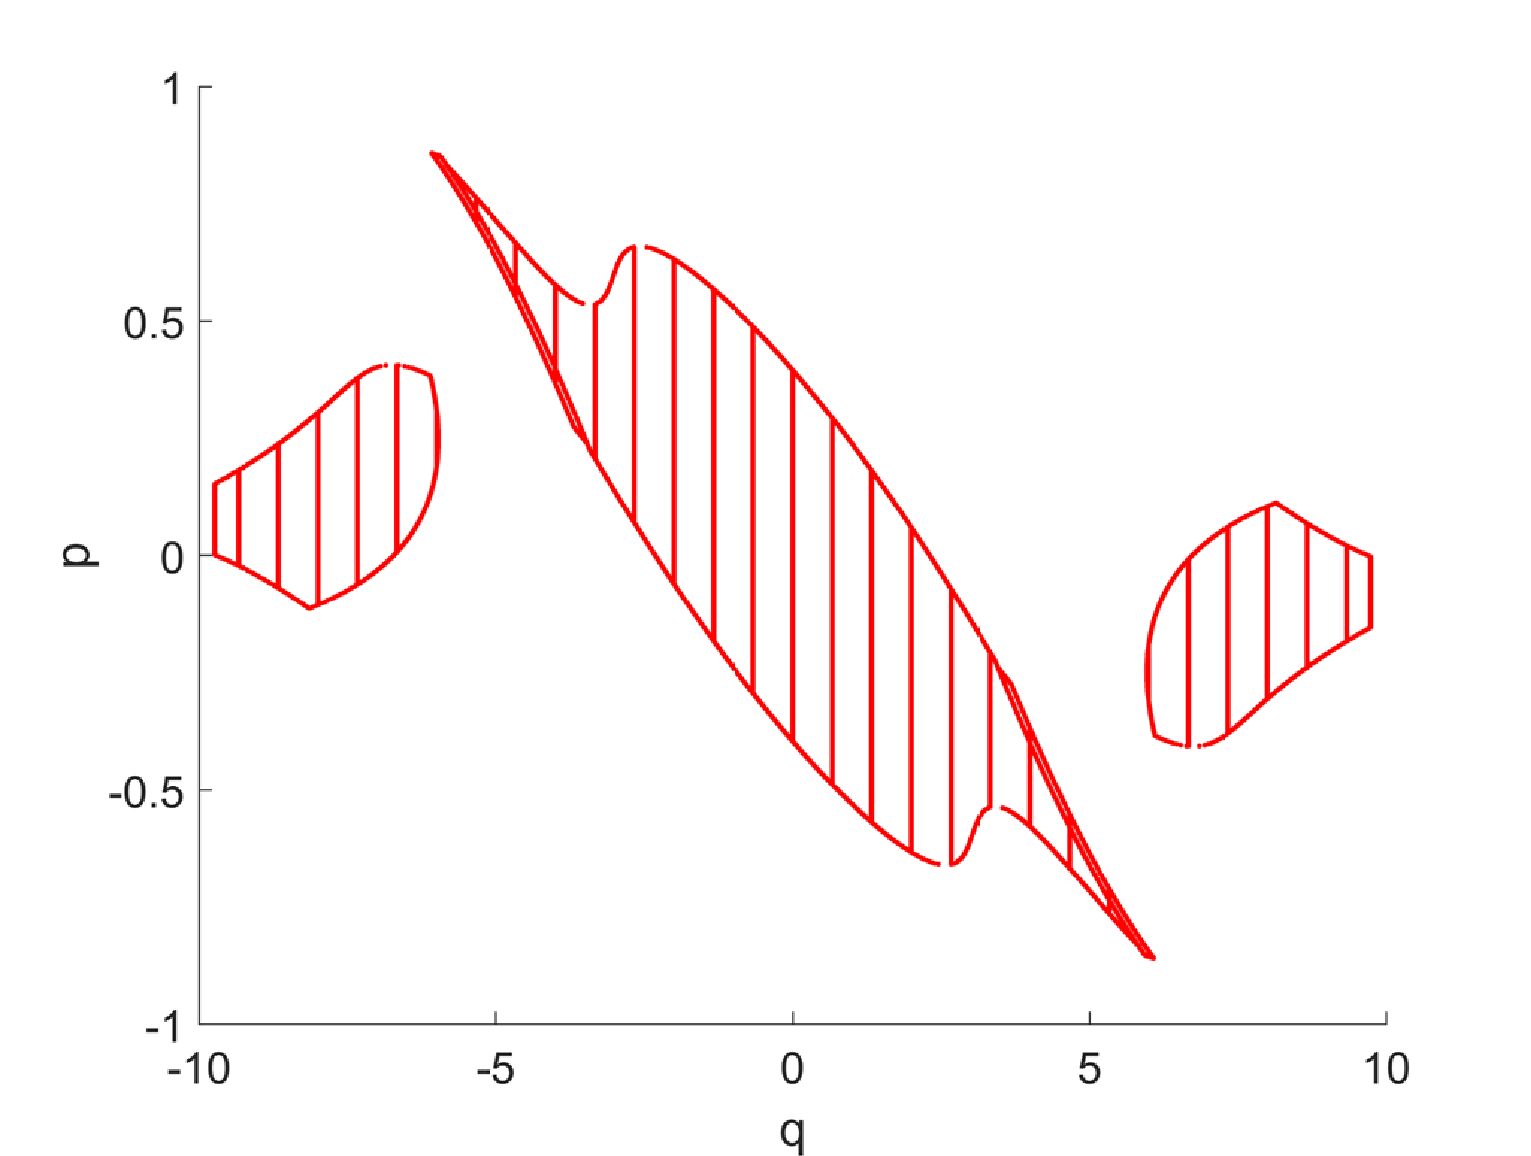
\includegraphics[width=0.7\textwidth]{boundaries_ray_mapping_tir2}
  \end{center}
  \caption{\textbf{Rays distribution at target PS of the TIR-collimator.}
 The $\variabile{q}$-axis is divided into $\textrm{Ni}=30$ bins, the $\variabile{p}$-axis is divided into $\nbin = 100$ bins. Considering only the rays that arrive to the source with the correct index of refraction ($\nline=1$), the regions with positive luminance are computed correctly.}
\label{fig:boundaries_TIR_ray_mapping1}
 \end{figure}
Figure \ref{fig:boundaries_TIR_ray_mapping1} shows that the rays on the boundaries $\partial$\set{R}{}{}$(\Pi_{\variabile{j}})$ are determined for every path $\Pi_{\variabile{j}}$ with $\variabile{j}\in\{1, \cdots, 5\}$. The ability of the inverse ray mapping method to recognize numerical noise gives the expectation that it is suitable for detect ghost stray light that is unwanted light which can reduce the performance of optical systems \cite{breault1995control}. Optical designers are interested in developing methods for minimization of stray light intensity \cite{grabarnik2015optical}. The inverse ray mapping could constitute an alternative approach for such purpose. 
\\ \indent Now we note that some rays inside the boundaries are still traced. This is related to the fact that we divide the target PS along the $\variabile{q}$-axis into $\textrm{Ni}=30$ bins. As a consequence, also the rays located at the end points of every bin are traced. \\
\indent The target ray mapping intensity $\hat{I}_{\textrm{RM}}$ is calculated using Equation \ref{eq:Ips}. The profile of $\hat{I}_{\textrm{RM}}$ obtained form inverse ray mapping with $\textrm{Ni}=30$ is depicted in Figure \ref{fig:intensity_tir_raymapping} with the red line. It is compared with the reference intensity (blue line) that is given by QMC ray tracing with $10^7$ rays. The picture shows that the inverse ray mapping method calculates the intensity correctly.
\begin{figure}[t]
  \begin{center}
  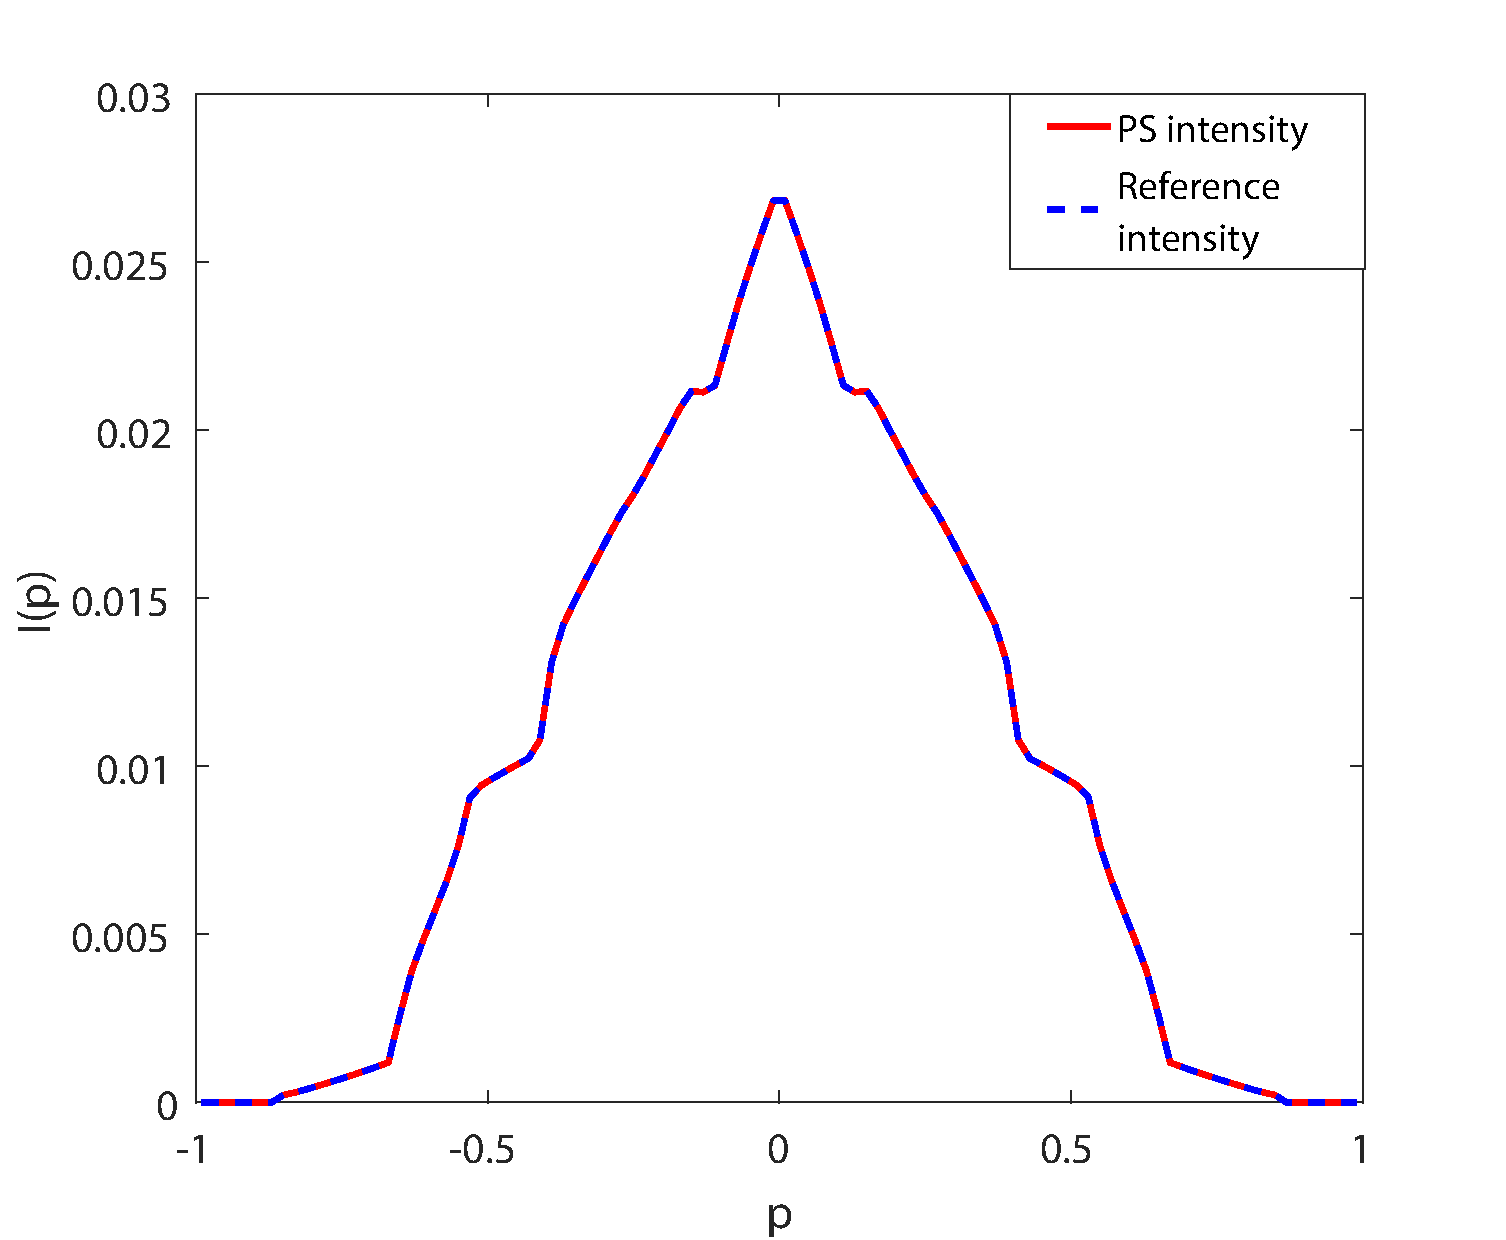
\includegraphics[width=0.7\textwidth]{intensity_tir_raymapping}
  \end{center}
  \caption{\textbf{Profile of the intensity for the TIR-collimator.}
 The ray mapping intensity is calculated dividing the $\variabile{q}$-axis into $\textrm{Ni}=30$ bins. The reference intensity is obtained from QMC ray tracing with $10^7$ rays.}
\label{fig:intensity_tir_raymapping}
 \end{figure}
\\ \indent 
Finally, we compare the inverse ray mapping with QMC ray tracing. The errors plot as a function of the CPU-time is shown in a logarithmic scale in Figure \ref{fig:error_tir_raymapping}. The approximation of the RM intensity $\hat{I}_{\textrm{RM}}$ is improved by increasing the number of bins $\textrm{Ni}$ in the partitioning $Q$. The approximated QMC intensity $\hat{I}_{\textrm{QMC}}$ is calculated several times gradually increasing the number of rays $\nrays$. Both the intensity are computed using the same number of bins $\nbin=100$ in the partitioning $P$ of the $\variabile{p}$-axis. The minimum ray mapping error is obtained with $\textrm{Ni}=100$ bins. While the minimum QMC error is achieved tracing $10^6$ rays. We observe that the minimal error obtained using the inverse ray mapping is of an order of magnitude of $10^{-6}$, while the minimum QMC error is of the order of $10^{-5}$. Furthermore, an extrapolation of QMC error shows that the inverse ray mapping is more than $20$ times faster compared to QMC.
\begin{figure}[t]
  \begin{center}
  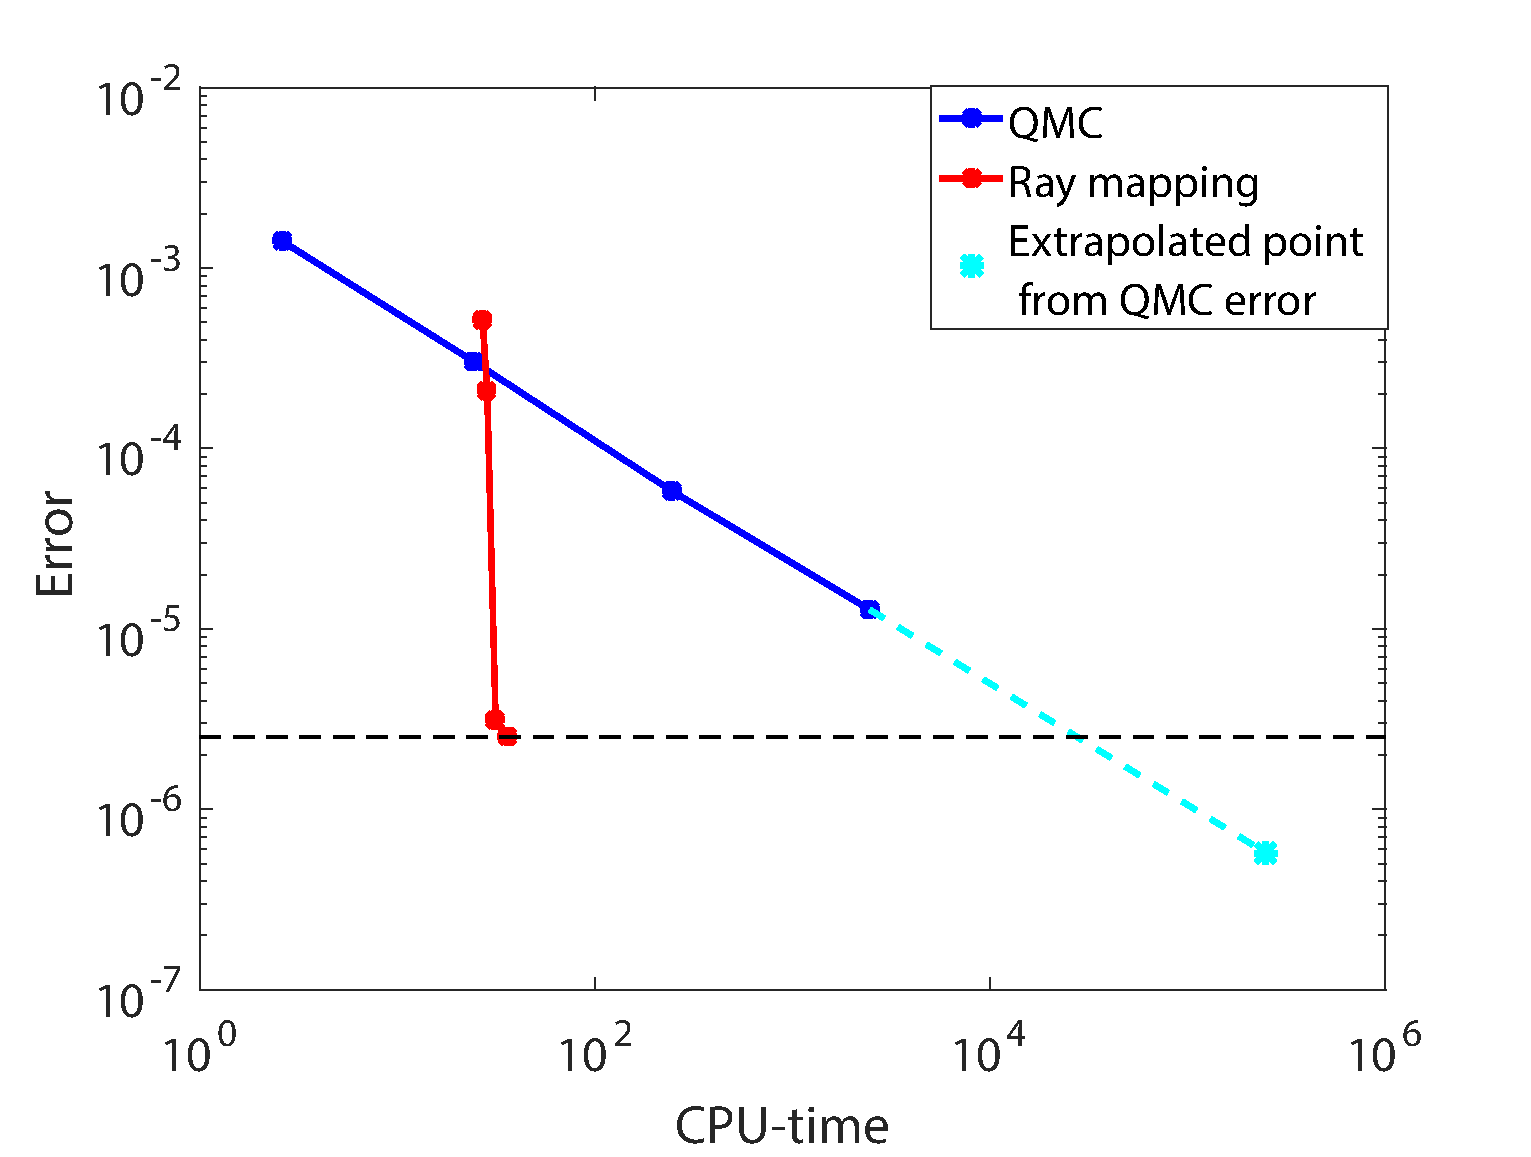
\includegraphics[width=0.7\textwidth]{error_tir_raymapping}
  \end{center}
  \caption{\textbf{Errors of ray mapping and QMC for the TIR-collimator.}
 The extended inverse ray mapping method is faster and more accurate than QMC ray tracing.}
\label{fig:error_tir_raymapping}
 \end{figure}
In Tables \ref{tab:ray_mapping_tir} the numerical results obtained for the inverse ray mapping are reported. The error values for QMC ray tracing were already reported in Chapter \ref{chap:triangulation} (Table \ref{tab:mc_error_triangulation}).
\begin{table}[t] 
\centering
\caption{\bf Errors of the PS intensity for the TIR-collimator}
\begin{tabular}{llllll}
 \hline  $\textrm{Ni}$\;  & RM error & $|\Delta U|$ & CPU-time (sec.)\\
  \hline 
 $5$    & $5.19\cdot10^{-4}$    & $1.6\cdot 10^{-1}$ & $269$  \\
$10$    & $2.09\cdot 10^{-4}$  & $2.8\cdot 10^{-2}$ & $284$   \\
$30$    & $3.15\cdot 10^{-6}$  & $5.7 \cdot 10^{-3}$ & $313$  \\
$100$  & $2.52\cdot 10^{-6}$  & $5.1 \cdot 10^{-3}$ & $359$  \\
 \hline
 \end{tabular}
 \label{tab:ray_mapping_tir}
 \end{table}
\\ \indent In the next section we present the method for a parabolic reflector.
\section{Results for a parabolic reflector}\label{sec:PR}
In this section we provide the results for the parabolic reflector in Figure \ref{fig:PR}.
This is a very challenging example of optical system. Indeed, the rays that propagate through such a system can reflect many times along the left and the right mirror. As we have seen using PS ray tracing, this leads to many different paths. Every path corresponds to a given number of reflections with each of the two reflector. In Chapter \ref{chap:triangulation} we found $17$ different paths for this parabolic reflector. Here, we apply the inverse ray mapping method to detect all this paths. \\ \indent
The target PS of the parabolic reflector is the rectangular \set{T}{}{}$=[-\variabile{b}, \variabile{b}]\times[-1,1]$ where $\variabile{b}=17$. Likewise, the TIR-collimator we divide the interval $[-\variabile{b}, \variabile{b}]$ in target PS into sub-intervals of the same length (bins). We remind the reader that we indicate with $\textrm{Ni}$ the number of bins in which we divide the interval $[-\variabile{b}, \variabile{b}]$ along the $\variabile{q}$-axis of \set{T}{}{} and with $\nbin$ the number of bins in which we divide the interval $[-1,1]$ along the $\variabile{p}$-axis. Considering a partitioning $Q = -\variabile{b}=\variabile{q}^{0}<\variabile{q}^{1}<\cdots<\variabile{q}^{\textrm{Ni}}=\variabile{b}$ of $[-\variabile{b}, \variabile{b}]$ and a direction $\variabile{p}\in[-1,1]$, the inverse ray mapping explained in Section \ref{sec:raymapping_explanation} is applied to every sub-interval $[\variabile{q}^{\textrm{k}}, \variabile{q}^{\textrm{k+1}}]\subset[-\variabile{b}, \variabile{b}]$ with $\textrm{k}=0, \cdots, \textrm{Ni}-1$ and for every direction $\variabile{p}\in[-1,1]$. To determine how many bins $\textrm{Ni}$ are needed for a good calculation of the target photometric variables, we employ the same idea of the TIR-collimator. The source \'{e}tendue $U_1$ is compared to several approximations of the \'{e}tendue at the target $U_{\textrm{t}}$ each of them is given by a different partitioning $Q$ of $[-\variabile{b}, \variabile{b}]$. For the parabolic reflector all the rays emitted from the source arrive at the target. Therefore, the exact \'{e}tendue as an area in PS is computed from Equation (\ref{eq:etenduesource}) obtaining $U=U_1=8$. The approximated target \'{e}tendue $U_{\textrm{t}}$ is given by Equation (\ref{eq:etendueintegraltarget}). In Figure \ref{fig:etendue_ray_mapping_pr_bin} we show the comparison between $U_1$ and several approximations of $U_{\textrm{t}}$ by gradually increasing the number of bins $\textrm{Ni}$ in the partitioning $Q$ while fixing the maximum number of multiple reflections to $30$. Increasing the bins $\textrm{Ni}$, the $U_{\textrm{t}}$ increases approaching to the exact value $U_1=8$. After the division into $\textrm{Ni}=4$ bins the improvement is slightly visible. We conclude that $\textrm{Ni}=4$ bins are enough to detect $30$ multiple reflections.
\begin{figure}[t]
  \begin{center}
  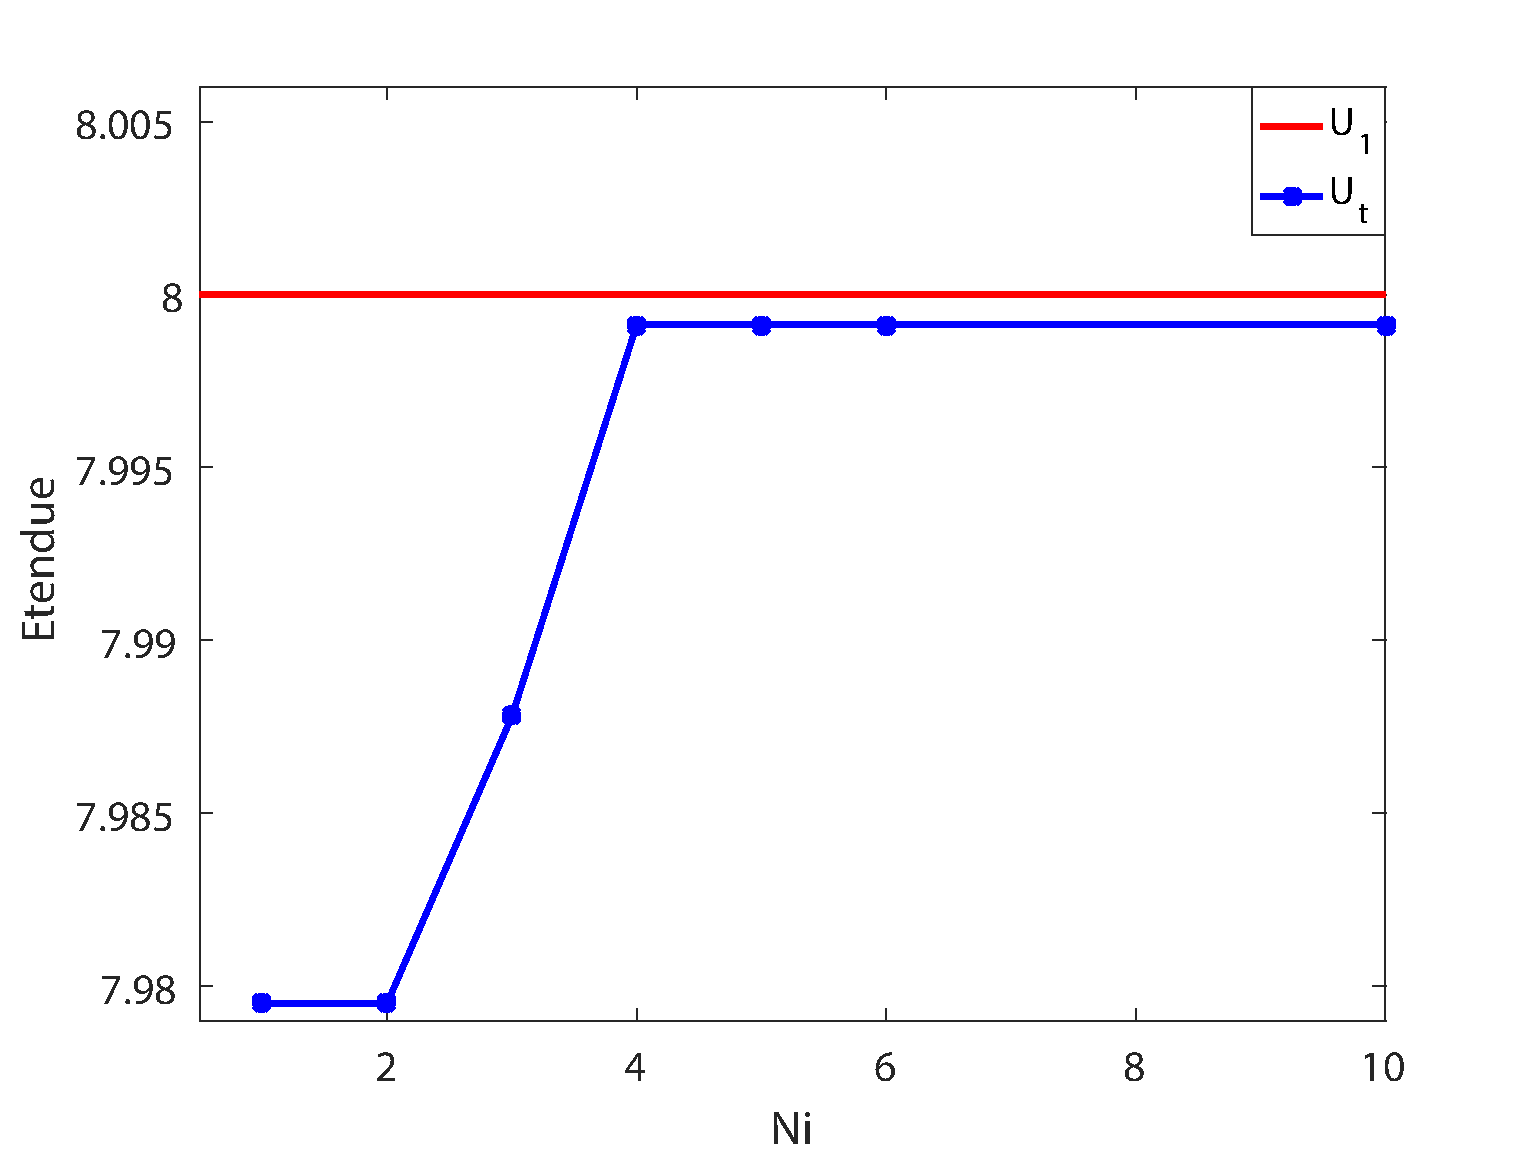
\includegraphics[width=0.7\textwidth]{etendue_ray_mapping_pr_bin}
  \end{center}
  \caption{\textbf{Comparison between the exact \'{e}tendue and the approximated target \'{e}tendue by increasing the number of bins $\textrm{Ni}$.}
 At most $30$ multiple reflections are considered. Increasing the bins $\textrm{Ni}$ gets closer to the exact value $U_1=8$.}
\label{fig:etendue_ray_mapping_pr_bin}
 \end{figure}
\\ \indent In Figure \ref{fig:boundaries_rays_pr_raymapping} we show rays distribution at the target PS obtained using the inverse ray mapping and considering $\textrm{Ni}=4$ and at most $30$ multiple reflections. The rays traced from the target to the source are depicted with the red dots. Most of the rays traced are located on the boundaries $\partial$\set{R}{}{}$(\Pi)$ of the regions with positive luminance. 
Only few rays are traced inside those regions. These are the rays located at the end points of every bin $[\variabile{q}^{\textrm{k}}, \variabile{q}^{\textrm{k}+1}]$ with $\textrm{k}=0, \cdots, \textrm{Ni}-1$. 
\begin{figure}[h]
  \begin{center}
  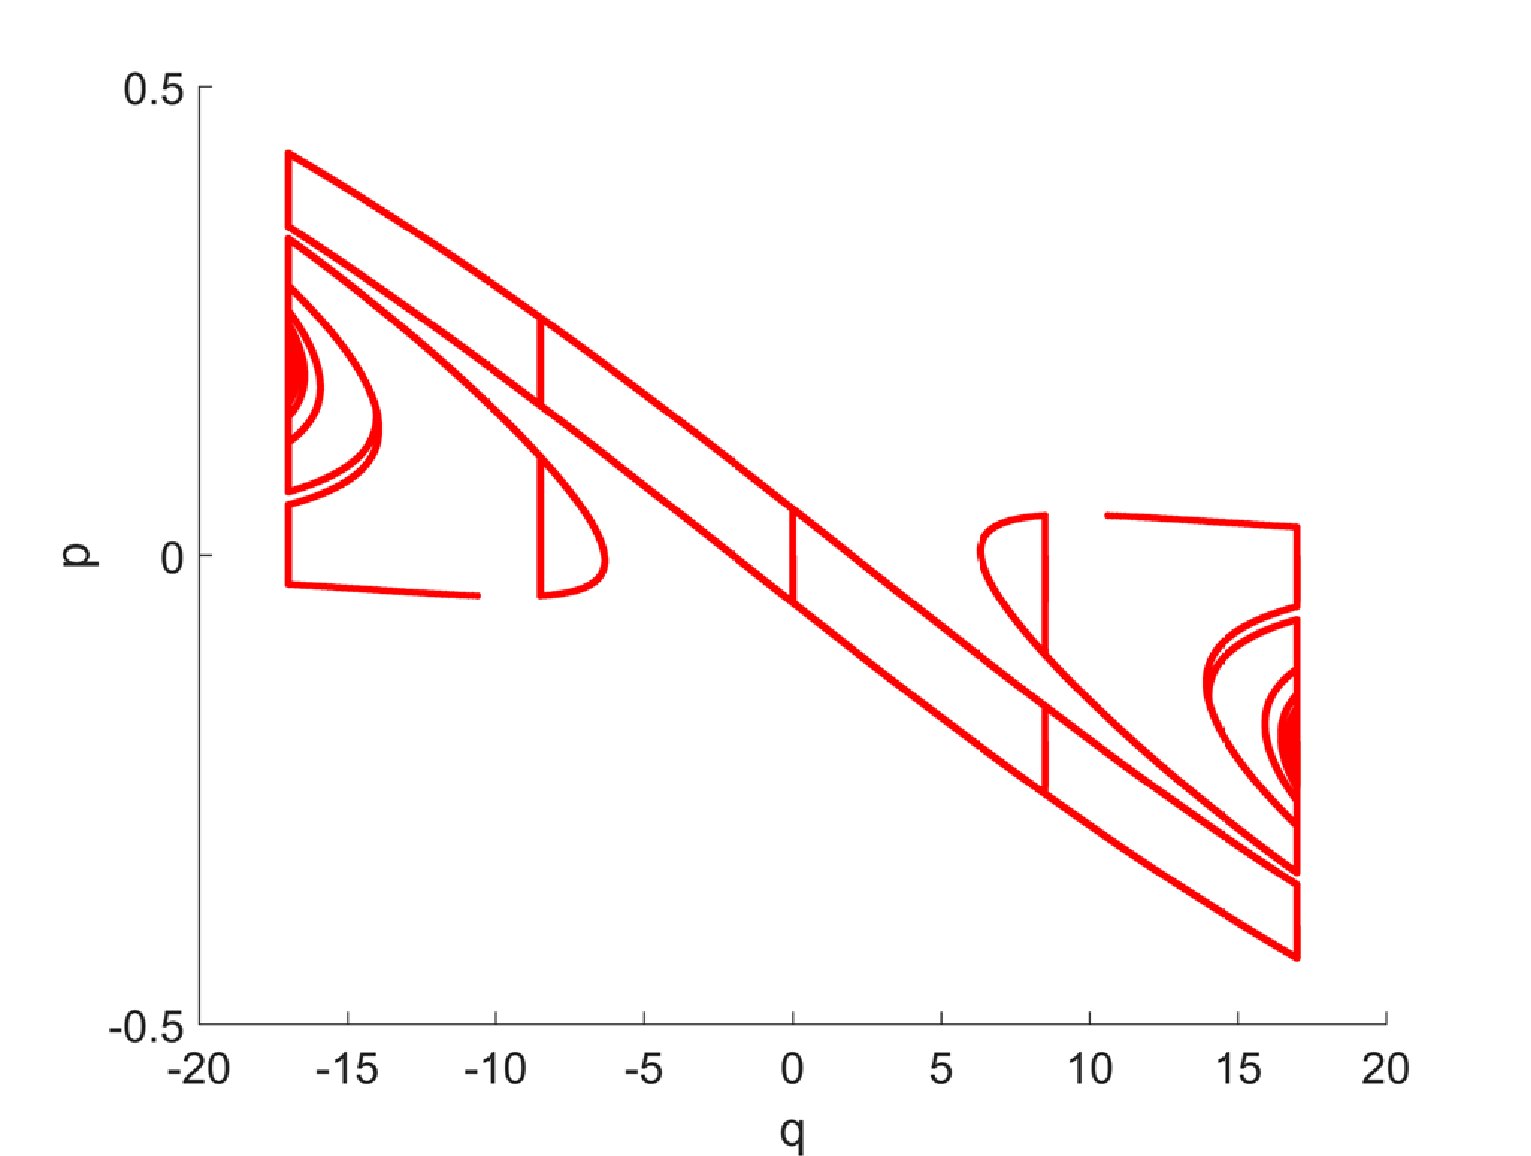
\includegraphics[width=0.7\textwidth]{boundaries_raymapping_pr}
  \end{center}
  \caption{\textbf{The red dots are the rays in target PS.}
 Considering $30$ multiple reflections, $\textrm{Ni}=4$ and $\nbin = 100$, only few rays using the inverse ray mapping.}
\label{fig:boundaries_rays_pr_raymapping}
 \end{figure}
\\ \indent
The inverse ray mapping method is able to detect $61$ different paths. Indeed $30$ multiple reflections can occur with the left reflector and $30$ with the right reflector. To those, the path that goes from the source to the target (no reflections with the reflectors) has to be added. For PS ray tracing we found at most $17$ paths for the same parabolic reflector. Hence, we claim that ray mapping is much more accurate than PS ray tracing. Also, we observe the procedure can be stopped when even more than $30$ multiple reflections are reached. The more reflections are considered the better accuracy is obtained. Again, to define a stopping criterion we use \'{e}tendue conservation. Fixing the number of bins $\textrm{Ni}=4$ and $\nbin=100$ and gradually increasing the number of multiple reflections we obtain that the approximated target \'{e}tendue $U_{\textrm{t}}$ changes as the blue line in Figure \ref{fig:etendue_pr_raymapping}. The horizontal red line represents the exact intensity $U = U_{1} = 8$. We note that the more reflections are considered the smaller value of $\Delta U = |U_1-U_{\textrm{t}}|$ is found (see also Table \ref{tab:ray_mapping_pr}). We observe that after around $30$ multiple reflections there is no significant improvement in the computation of $U_{\textrm{t}}$. This is due to the fact that only few rays follow multiple reflections and therefore, they do not give a significant contribution to the total \'{e}tendue (the regions in PS formed by those rays are very small compared to the entire PS). This gives the insight that the inverse ray mapping has a good accuracy when around $30$ multiple reflections and $\textrm{Ni}=4$ bins are taken into account.
\begin{figure}[h]
  \begin{center}
  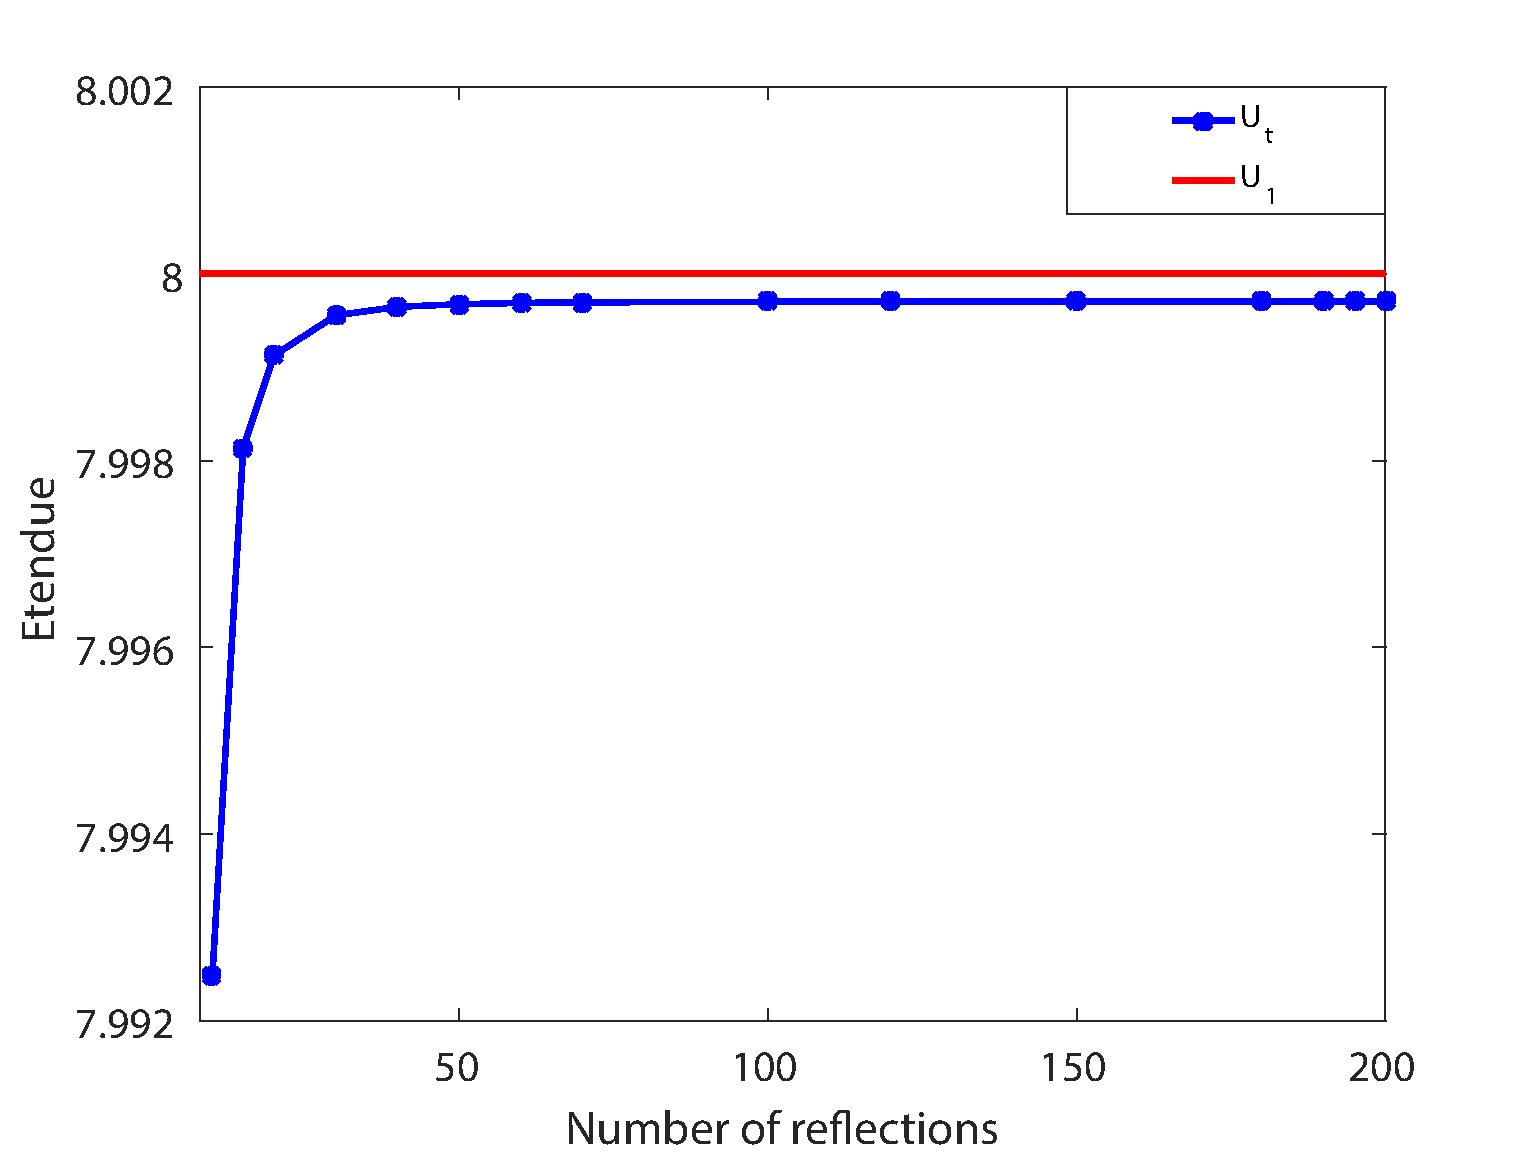
\includegraphics[width=0.7\textwidth]{etendue_pr_raymapping}
  \end{center}
  \caption{\textbf{Comparison between the exact \'{e}tendue and the approximated target \'{e}tendue by increasing the number of multiple reflections.}
Fixing the number of bins along the $\variabile{q}$-axis $\textrm{Ni}=4$ and increasing the number of reflections considered, the \'{e}tendue increases approaching to the exact value $U_1=8$.}
\label{fig:etendue_pr_raymapping}
 \end{figure}
Once a stopping criterion is established, ray mapping is run and the rays on the boundaries are determined. Finally, the target intensity is calculated from Equation (\ref{eta2}). 
\\ \indent In Figure \ref{fig:intensity_pr_raymapping} both the ray mapping intensity (red line) and the reference intensity (dotted blue line) are shown. The ray mapping intensity $\hat{I}_{\textrm{RM}}$ is obtained considering at most $30$ multiple reflections, $\textrm{Ni}=4$ and $\nbin = 100$. The reference intensity $\hat{I}_{\textrm{ref}}$ is given by QMC ray tracing with $10^8$ rays and $\nbin = 100$. The two intensities overlap.
\begin{figure}[t]
  \begin{center}
  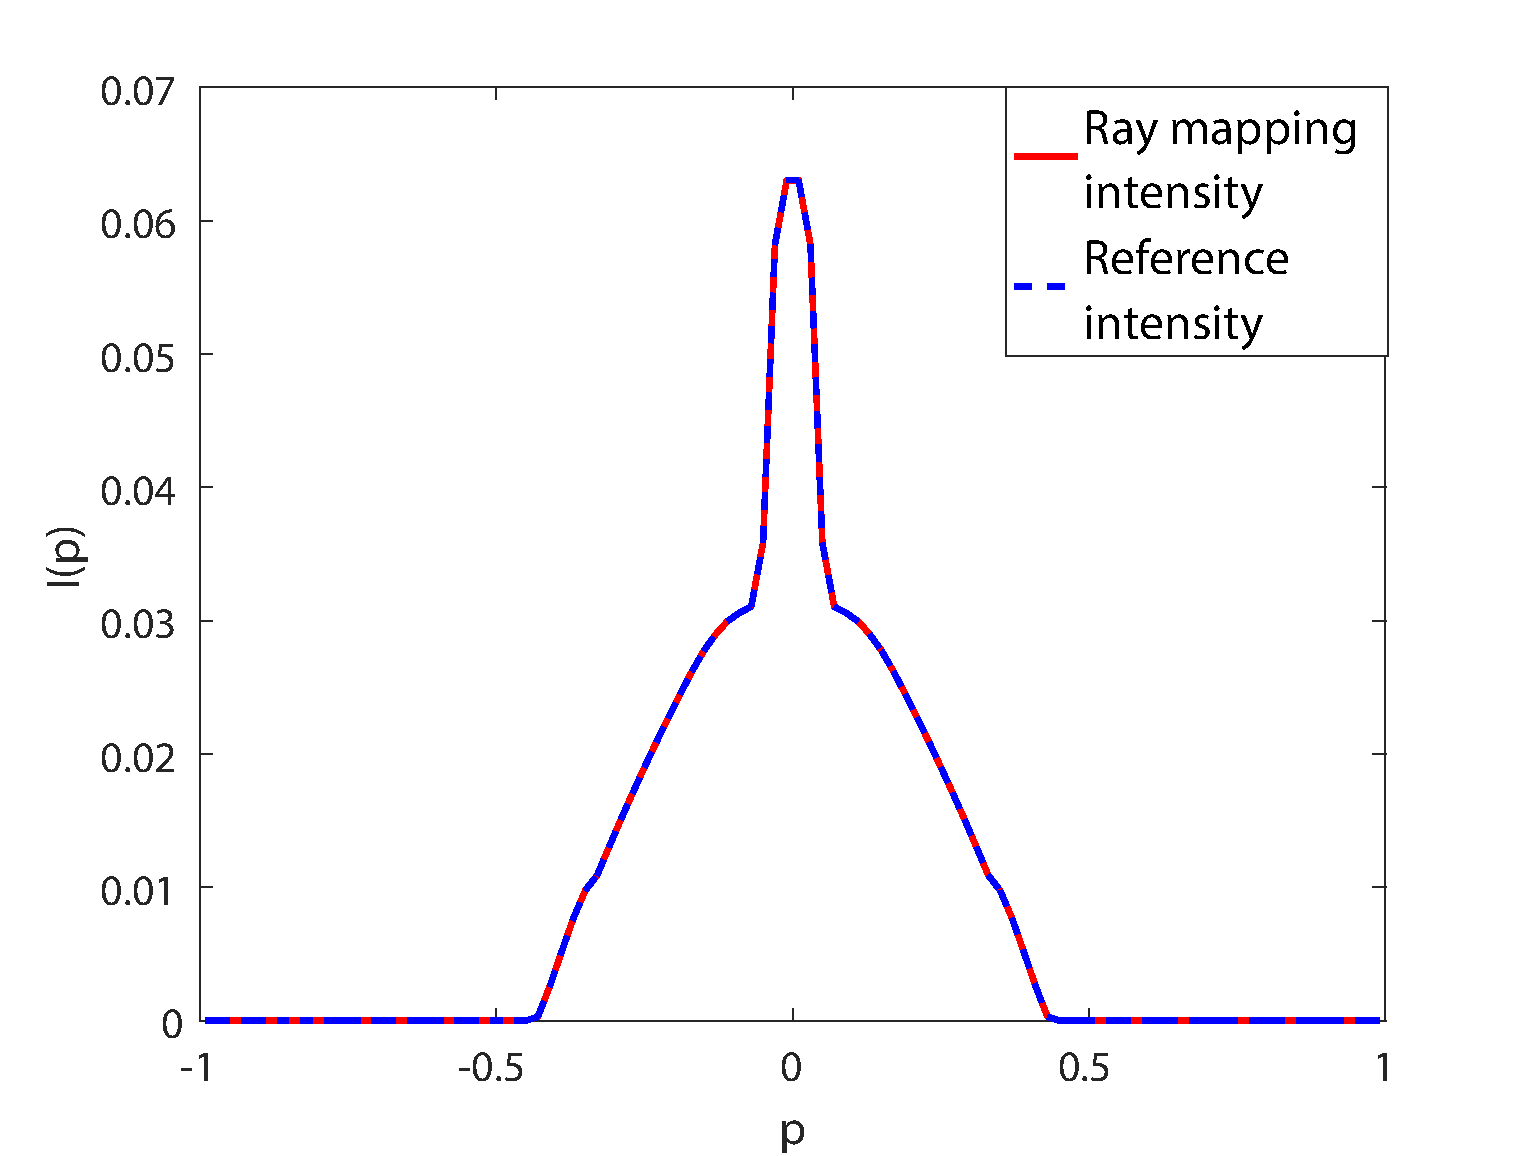
\includegraphics[width=0.7\textwidth]{intensity_pr_raymapping}
  \end{center}
  \caption{\textbf{Ray mapping intensity compared to a reference intensity.}
The ray mapping error is calculated considering $\textrm{Ni}=4$ and at most $30$ multiple reflections. The reference intensity is obtained by running QMC ray tracing with $10^8$ rays.}
\label{fig:intensity_pr_raymapping}
 \end{figure}
\\ \indent
To conclude we calculate the errors between the approximated intensity $\hat{I}_{\textrm{A}} (\textrm{A}=\textrm{RM}, \textrm{QMC})$ and the reference intensity $\hat{I}_{\textrm{ref}}$. From the results in Figure \ref{fig:error_raymapping_pr} we observe that the RM error (red line) converges faster than QMC error (blues line) as long as an error of an order of $10^{-6}$ is desired. Ray mapping results to be around $20$ times faster than QMC ray tracing. Furthermore, it is much more accurate than QMC. Our method is able to detect \textit{all} the possible paths that can occur. The procedure is stopped when $200$ multiple reflections are reached. Our expectation is that, increasing the number of multiple reflections and the number of bins $\textrm{Ni}$, the accuracy can be improved even more.
\begin{figure}[h]
  \begin{center}
  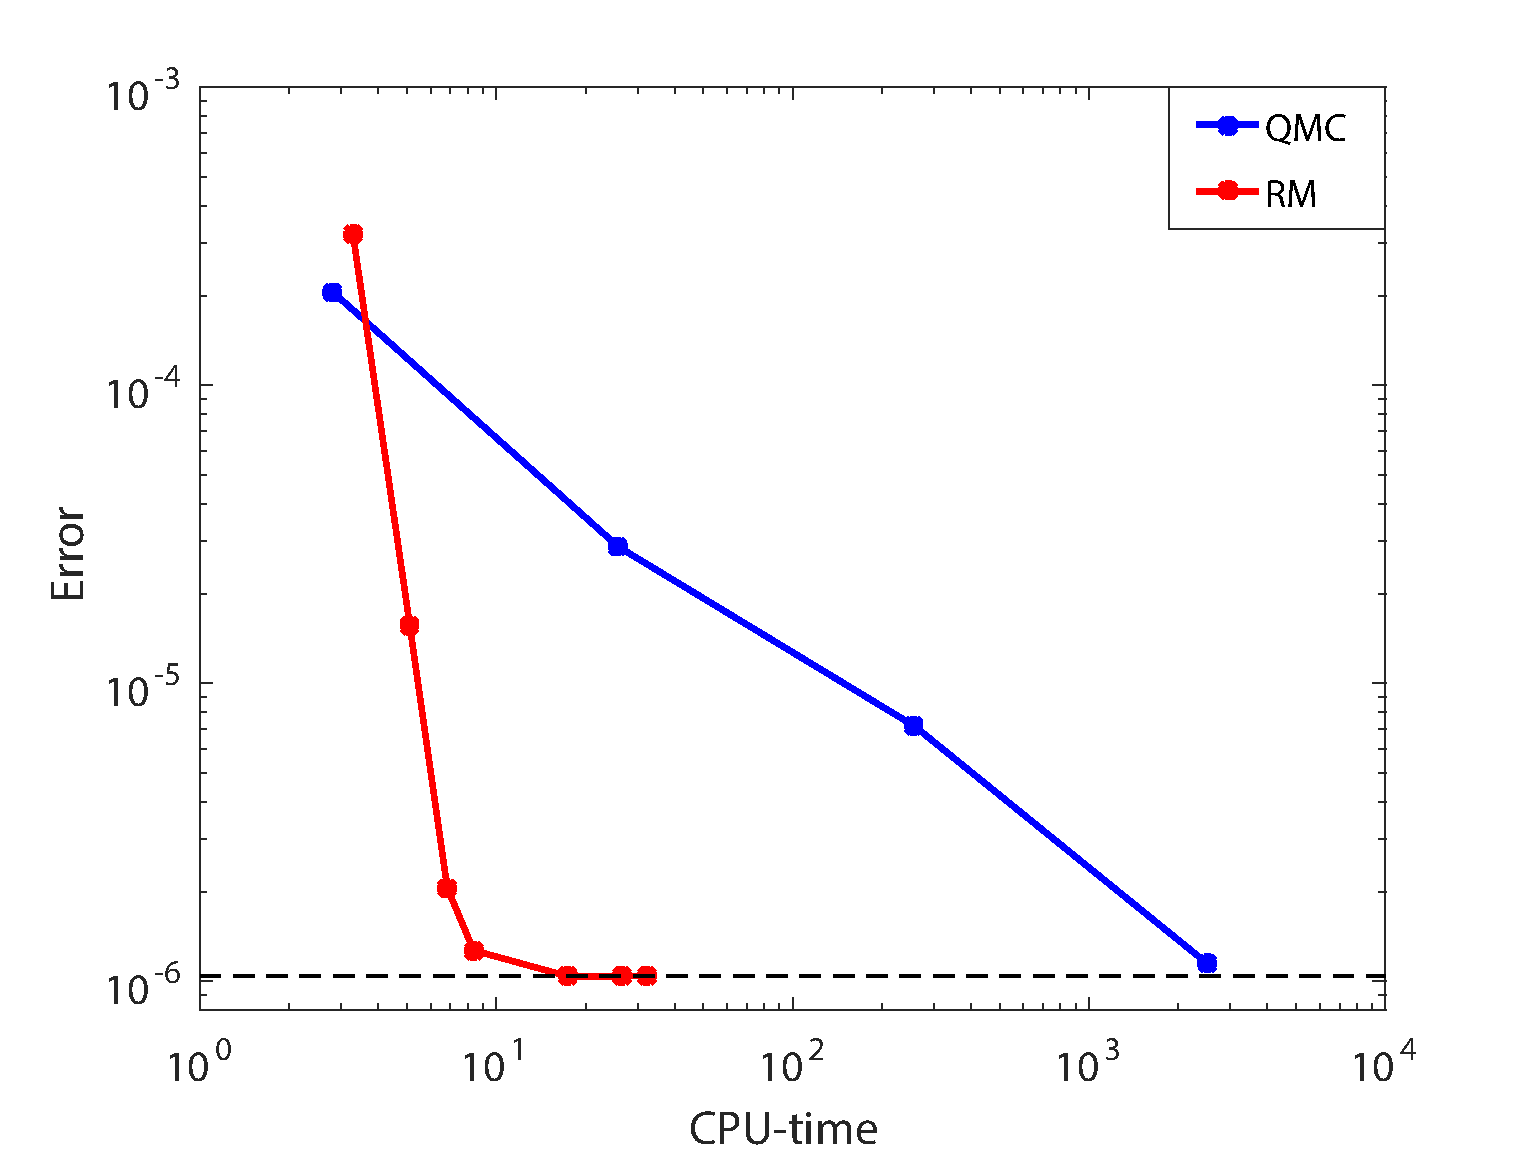
\includegraphics[width=0.7\textwidth]{error_pr_raymapping}
  \end{center}
  \caption{\textbf{Errors of ray mapping and QMC for the parabolic reflector.}
The ray mapping error decreases by increasing the number of reflections considered.
The QMC error reduces by tracing more rays.
 The extended inverse ray mapping method is faster and more accurate than QMC ray tracing.}
\label{fig:error_raymapping_pr}
 \end{figure}
In Tables \ref{tab:ray_mapping_pr} and \ref{tab:qmc_raymapping_pr} these numerical results are reported.
\begin{table}[t] 
\centering
\caption{\bf Errors of the ray mapping intensity for the parabolic reflector}
\begin{tabular}{llllll}
 \hline  Number of\\
 reflections\;  & RM error & $|\Delta U|$ & CPU-time (sec.)\\
  \hline 
 $5$      & $1.74\cdot 10^{-1}$  & $3.222\cdot10^{-4}$& $3.28$  \\
$10$      & $7.52\cdot 10^{-3}$ & $1.555\cdot 10^{-5}$& $5.11$   \\
$20$      & $9.00 \cdot 10^{-4}$ & $2.059\cdot 10^{-6}$& $6.83$  \\
 $30$    & $5.00 \cdot 10^{-4}$ & $1.269\cdot 10^{-6}$ & $8.38$  \\
$100$    & $2.99 \cdot 10^{-4}$ & $1.038\cdot 10^{-6}$ & $17.49$  \\
$150$    & $2.96 \cdot 10^{-4}$ & $1.039\cdot 10^{-6}$ & $26.38$  \\
$200$    & $2.95 \cdot 10^{-4}$ & $1.039\cdot 10^{-6}$ & $32.21$  \\
 \hline
 \end{tabular}
 \label{tab:ray_mapping_pr}
 \end{table}
\begin{table}[t] 
\centering
\caption{\bf Errors of the QMC intensity for the parabolic reflector}
\begin{tabular}{lllll}
 \hline  $\nrays$\;  & QMC error & CPU-time (sec.)\\
  \hline 
$10^4$     & $2.05\cdot 10^{-4}$   & $2.81$  \\
$10^5$     & $2.87\cdot 10^{-5}$   & $25.81$   \\
$10^6$     & $7.18 \cdot 10^{-6}$  & $257.54$  \\
$10^7$     & $1.15 \cdot 10^{-6}$  & $2491.32$  \\
 \hline
 \end{tabular}
 \label{tab:qmc_raymapping_pr}
 \end{table}
\section{Conclusions}
In this chapter we present the extension of the analytic ray mapping method to system formed by curved lines. Employing the inverse ray tracing and a bisection procedure in target PS, an inverse map from the target to the source is constructed such that all the possible paths that the rays can follow are determined. The extended ray mapping method is able to detect the rays located on the boundaries of the regions formed by rays that follow the same path. From these rays the target intensity is calculated. 
\\ \indent
We presented to examples of optical systems: the TIR-collimator and a parabolic reflector. In both cases the target PS is divided into bins and the procedure is applied to each bin. A stopping criterion based on \'{e}tendue conservation is developed to determine the number of bins needed to obtain a good accuracy. For the TIR-collimator we noticed that the method is able to detect rays that follow an \textit{unphysical} path due to numerical error. This gives the expectation that the inverse ray mapping can be used also for detecting ghost stray light.
For the parabolic reflector, many paths can occur along the reflectors. Etendue conservation is used again to determine the number of multiple reflections to be considered. The target intensity is computed for both the systems and it is compared with a reference intensity given by QMC ray tracing with a large number of rays. The results shown that the method is able to detect all the possible paths tracing few rays through the system. Comparing our method to QMC ray tracing, significant advantages are observed in the accuracy and the computational time for both the optical systems analyzed.
% Explain the results
\\ \indent In the next chapter we explain how to apply the method to systems with Fresnel reflection. We present the method for a system formed by the source, an ideal lens and the target. 













